\documentclass[12pt,a4paper,twoside,openany]{report}

\usepackage[portuguese,main=english]{babel}
\usepackage{fontspec}
\usepackage{csquotes} % Recommended for biblatex
\usepackage{hyperref}

\usepackage[noend]{algpseudocode}

% NewsGotT is the University of Minho text face (RT-80/2026, item 1).
% The files in assets/fonts/ include real italic and bold italic.
\setmainfont{NewsGotT}[
  Path=assets/fonts/,
  Extension=.ttf,
  UprightFont=ngottr,
  BoldFont=ngottb,
  ItalicFont=ngottri,
  BoldItalicFont=ngottbi,
  Ligatures=TeX
]
\newfontfamily\NewsGotTLight{NewsGotTLig}[
  Path=assets/fonts/,
  Extension=.ttf,
  UprightFont=ngottl,
  ItalicFont=ngottli,
  Ligatures=TeX
]

% NewsGotT has no ė, ń or Ż. Names in the bibliography use them.
% Latin Modern supplies only those glyphs; the entries themselves are unchanged.
\usepackage{newunicodechar}
\newfontfamily\GlyphFallback{lmroman10-regular.otf}[
  BoldFont=lmroman10-bold.otf,
  ItalicFont=lmroman10-italic.otf,
  BoldItalicFont=lmroman10-bolditalic.otf,
  Ligatures=TeX
]
\newunicodechar{ė}{{\GlyphFallback ė}}
\newunicodechar{ń}{{\GlyphFallback ń}}
\newunicodechar{Ż}{{\GlyphFallback Ż}}

\usepackage{amsmath,amssymb}
\usepackage[a4paper,margin=2.5cm]{geometry}
\usepackage{booktabs}
\usepackage{graphicx}
\usepackage{float}
\usepackage{pdfpages}
\usepackage{titlesec}
\usepackage{multirow}
\usepackage{tabularx}
\usepackage{tabulary}
\usepackage{url}
\usepackage[bottom]{footmisc}
\usepackage[nohyperlinks]{acronym}
\usepackage{listings}

\usepackage{pdflscape} % For landscape pages
\usepackage{afterpage} % For page control

\usepackage{mathtools}
\usepackage{chngcntr}

% RT-80/2026, item 16: 1.5 line spacing in the body.
% The reference list sets this back to 1 via \bibfont.
\linespread{1.5}
% Long file names in \texttt cannot hyphenate. A little stretch avoids
% overfull lines without changing the wording.
\setlength{\emergencystretch}{2em}

% RT-80/2026, item 16: footnotes are 8 pt. Leading is 1.5 times that size.
\renewcommand{\footnotelayout}{\fontsize{8pt}{12pt}\selectfont}

% RT-80/2026, item 17: figures and tables are numbered 1 to N, not by chapter.
\counterwithout{figure}{chapter}
\counterwithout{table}{chapter}

\hypersetup{
    colorlinks=false,
    linktoc=all,
    hidelinks
}

% Load biblatex with biber and authoryear style
\usepackage[
  backend=biber,
  style=authoryear,
  uniquelist=false,
  maxcitenames=2,
  mincitenames=1
]{biblatex}
\addbibresource{references.bib} % Ensure this file exists

% Remove bold or small caps from names
\renewcommand*{\mkbibnamegiven}[1]{#1}
\renewcommand*{\mkbibnamefamily}[1]{#1}
\renewcommand*{\mkbibnameprefix}[1]{#1}
\renewcommand*{\mkbibnamesuffix}[1]{#1}

% Set the delimiter between multiple citations
\renewcommand*{\multicitedelim}{\addsemicolon\space}

% Set the delimiter between name and year
\renewcommand*{\nameyeardelim}{\addcomma\space}

% RT-80/2026, item 16: the reference list may be single-spaced.
\renewcommand{\bibfont}{\normalfont\normalsize\linespread{1}\selectfont}

\newcommand{\term}[1]{\ensuremath{\mathsf{#1}}}
\newcommand{\nterm}[1]{\ensuremath{\langle\mathit{#1}\rangle}}
\newcommand{\produces}{\ensuremath{::=}}
\newcommand{\alt}{\ensuremath{\mid}}

% Remove any formatting from \parencite
\DeclareFieldFormat[parencite]{citehyperref}{#1}

% Included cover sheets use fitpaper, which changes the page size.
% Body pages stay A4.
\newcommand{\RestoreAFour}{%
  \setlength{\paperwidth}{210mm}%
  \setlength{\paperheight}{297mm}%
  \setlength{\pdfpagewidth}{210mm}%
  \setlength{\pdfpageheight}{297mm}%
}

% Lists of figures and tables use the same section heading as the rest of
% the front matter. \listoffigures would open with \chapter*, and a second
% page break in front of that ships a blank page.
\makeatletter
\newcommand{\uminholist}[2]{%
  \clearpage
  \phantomsection
  \addcontentsline{toc}{section}{#1}%
  \section*{#1}%
  \@starttoc{#2}%
}
\makeatother

% Missing results images keep their figure environment and caption.
\newcommand{\includefig}[2][]{%
  \IfFileExists{#2}{%
    \includegraphics[#1]{#2}%
  }{%
    \PackageWarning{thesis}{Missing figure file #2}%
    \setlength{\fboxsep}{8pt}%
    \fbox{%
      \begin{minipage}[c][0.30\textheight][c]{0.90\linewidth}
        \centering
        \textbf{TODO(Dong): missing figure file.}\\[0.6em]
        \texttt{\detokenize{#2}}\\[0.6em]
        The figure environment and its caption are unchanged.
        Put the image at this path and rebuild.
      \end{minipage}%
    }%
  }%
}

\begin{document}
\raggedbottom
\pagestyle{plain}

% Outer cover. Left as a PDF. Not part of the numbered sequence.
\hypersetup{pageanchor=false}
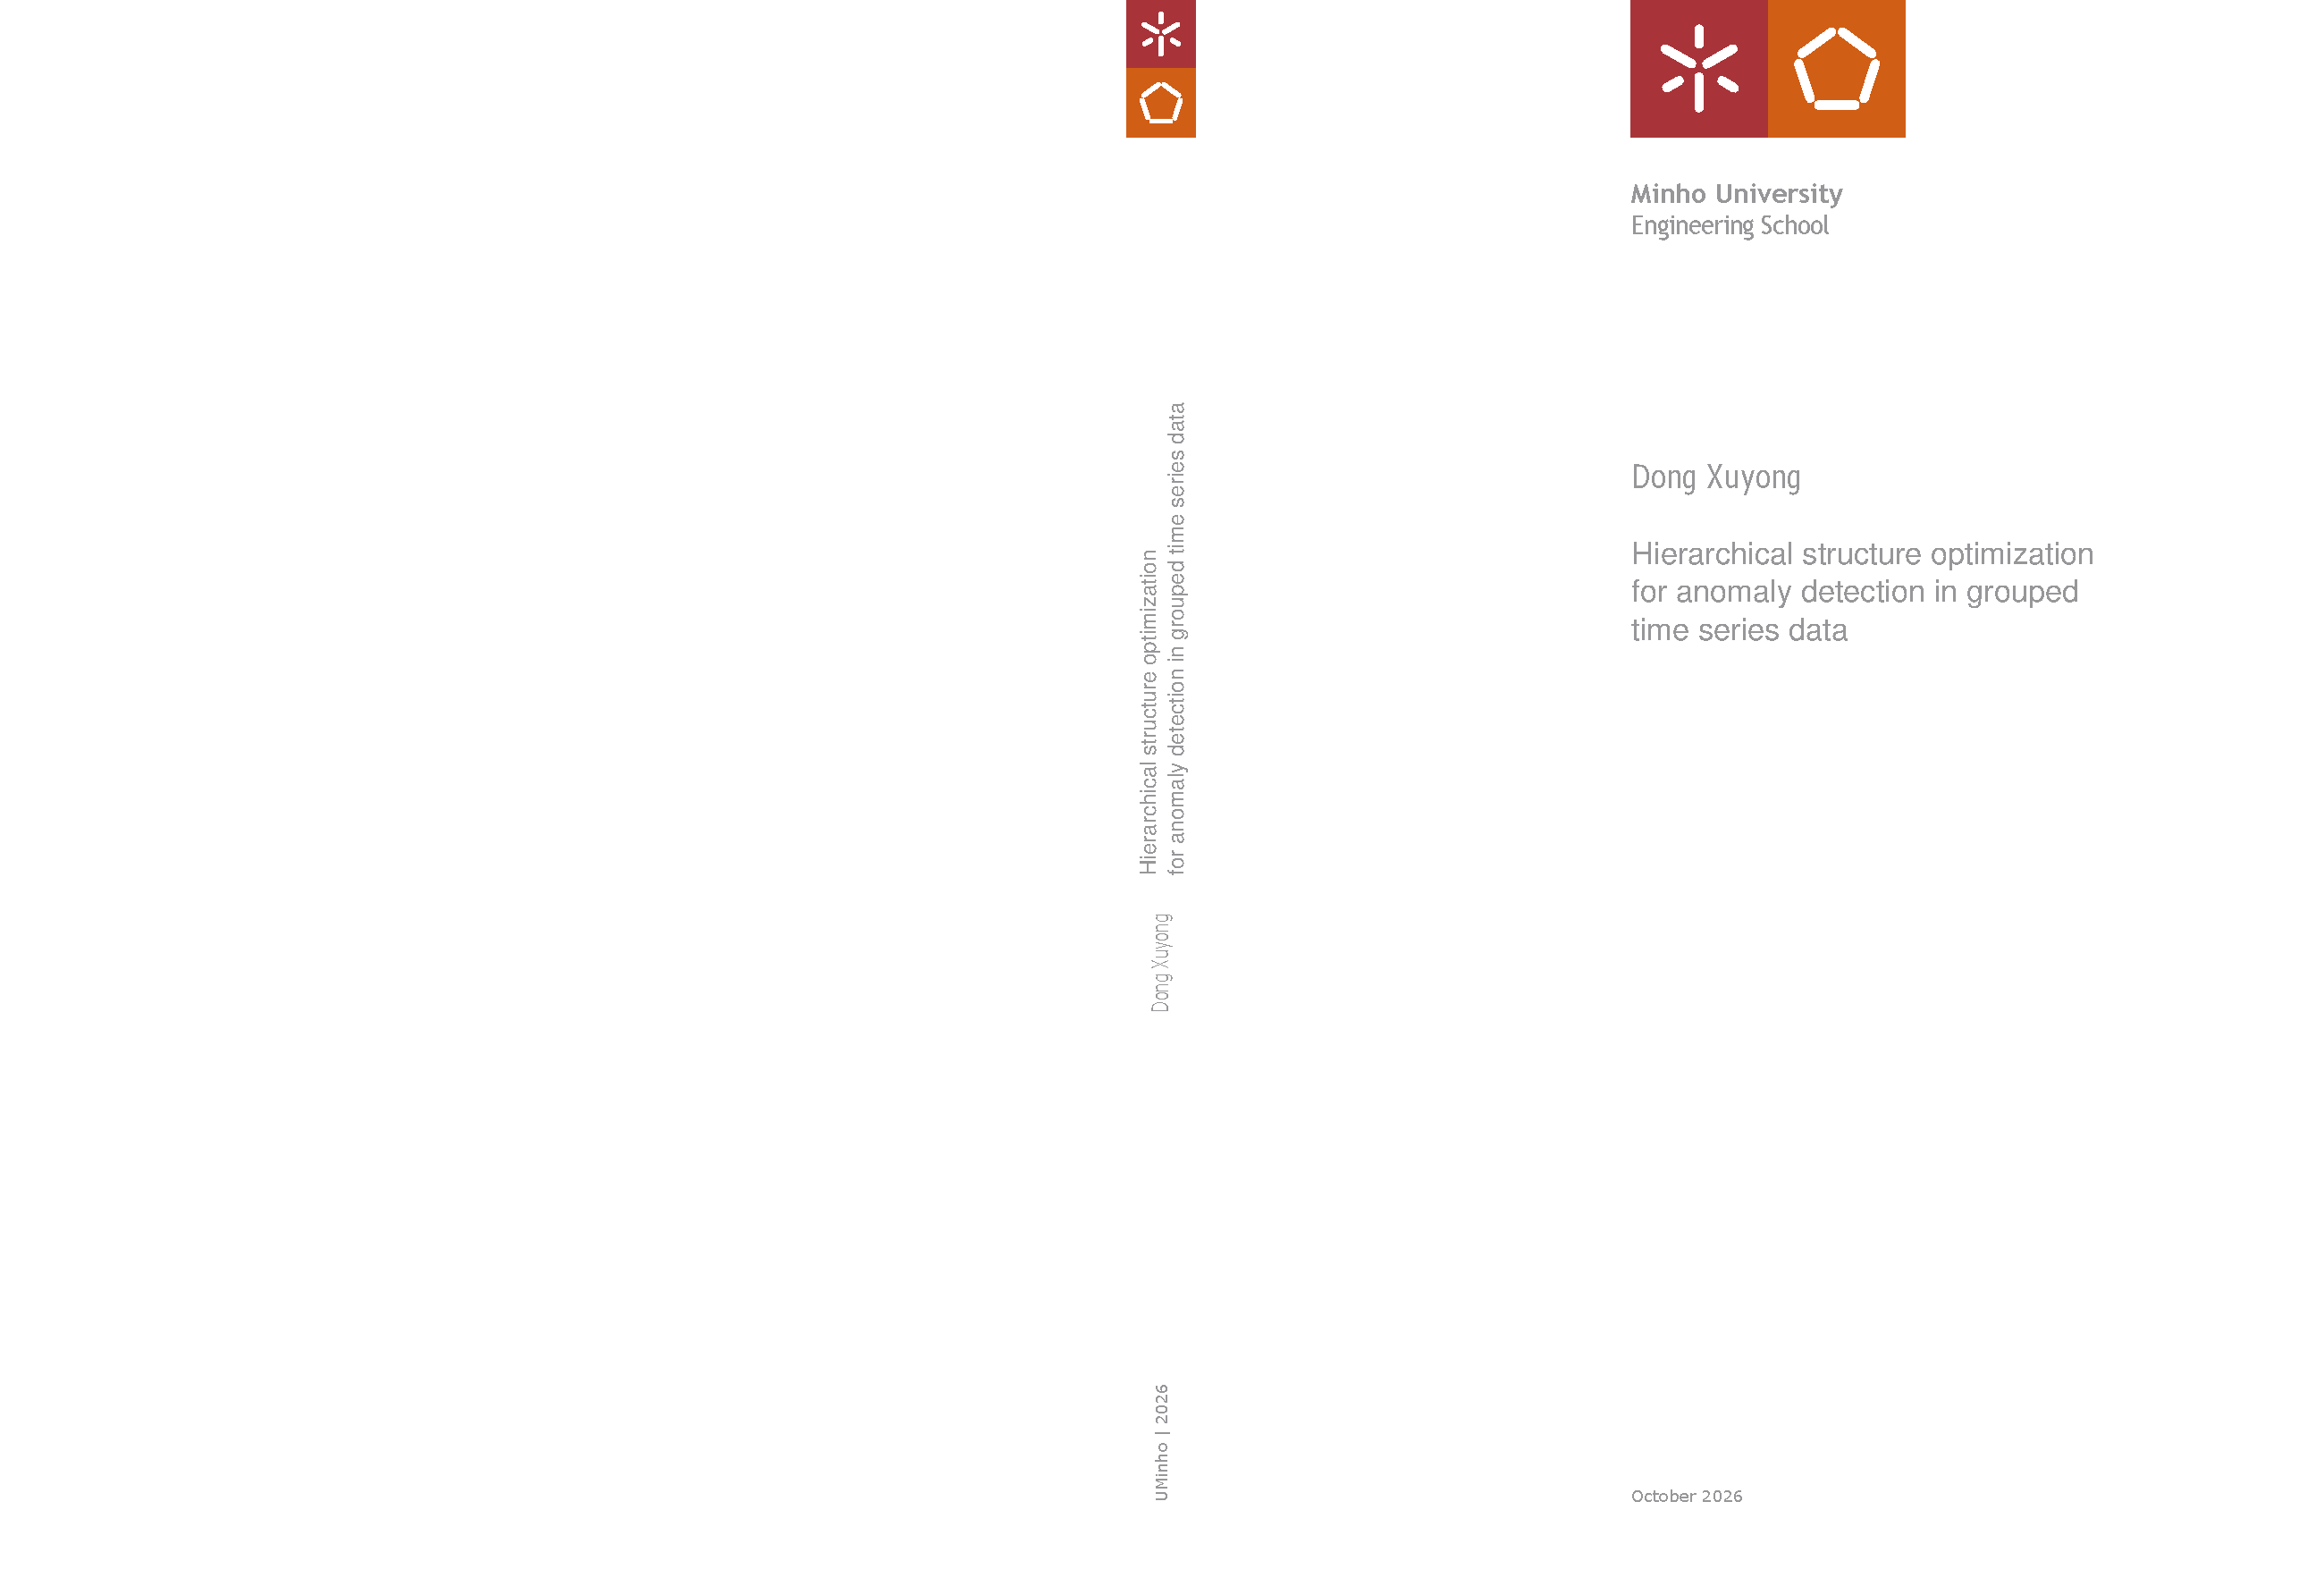
\includepdf[fitpaper,pages=-]{assets/pdf/capa2.pdf}
\RestoreAFour

% Title page (folha de rosto): counted as roman i, number not printed.
% pdfpages already applies an empty page style to included sheets.
\hypersetup{pageanchor=true}
\pagenumbering{roman}
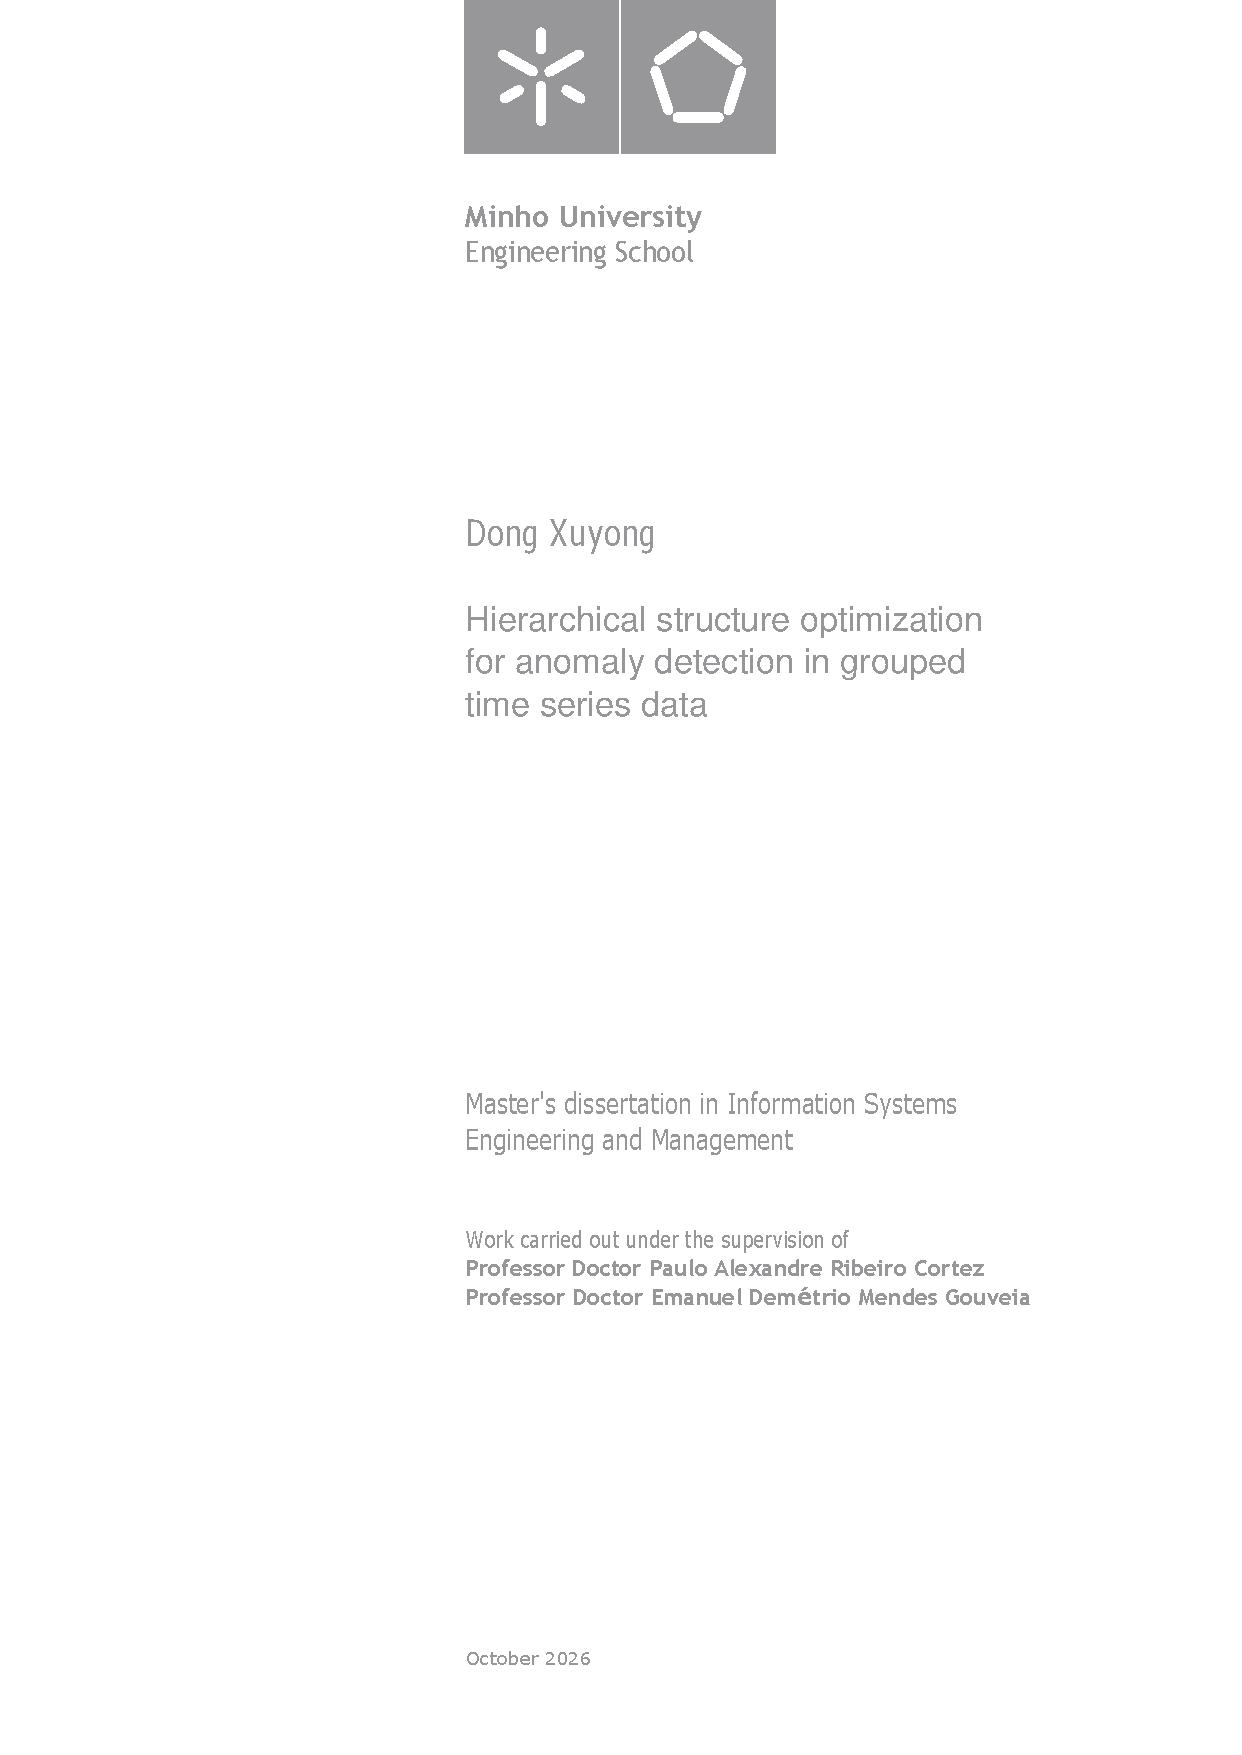
\includepdf[fitpaper,pages=-]{assets/pdf/capa1.pdf}
\RestoreAFour

% 3-literature-review.tex is included at the end of 2-theory-background.tex.

\cleardoublepage
\phantomsection
\section*{Copyright and terms of use of the work by third parties}

This is an academic work that can be used by third parties as long as internationally accepted rules and good practices are respected with regard to copyright and related rights.
The work may be used under the terms of the licence below.
If a use is not covered by that licence, the user should contact the author through the RepositóriUM of the University of Minho.

\noindent\textbf{Licence granted to users of this work}\\
Attribution-NonCommercial\\
CC BY-NC\\
\url{https://creativecommons.org/licenses/by-nc/4.0/}

\cleardoublepage
\phantomsection
\section*{Acknowledgements}

Looking back on the work that led to this dissertation, I am deeply grateful to the people whose guidance, support and encouragement made it possible.

My deepest thanks go to my supervisor, Professor Doctor Paulo Alexandre Ribeiro Cortez, who has been a constant source of motivation throughout this research.
His knowledge, rigour and dedication to academic excellence guided my work at every stage, and I learned a great deal from his teaching and advice during the master's programme and the whole period of this study.

I am also grateful to my co-supervisor, Professor Doctor Emanuel Demétrio Mendes Gouveia, for his insights and encouragement.
His perspective and feedback were essential in shaping and broadening the scope of this work, and the collaborative atmosphere he fostered contributed greatly to my academic growth.

I also thank the telecommunications operator that made the network data available, without which this study would not have been possible, and the developers of the open-source tools on which this work is built, in particular PonyGE2 and STUMPY.

Finally, I thank my family and friends for their unconditional love, patience and encouragement throughout this journey.

\cleardoublepage
\phantomsection
\section*{Statement of integrity}

I hereby declare having conducted this academic work with integrity.
I confirm that I have not used plagiarism or any form of undue use of information or falsification of results along the process leading to its elaboration.
I further declare that I have fully acknowledged the Code of Ethical Conduct of the University of Minho.

\cleardoublepage
\phantomsection
\section*{Abstract}
\addcontentsline{toc}{section}{Abstract}

This dissertation focuses on anomaly detection in grouped telecommunications time-series data from a real network.
Modern telecommunications networks generate large volumes of traffic that must be monitored to detect anomalous behaviour that can affect service reliability, capacity provisioning, and operational decision-making.
These datasets are structured along several categorical dimensions, which creates many possible aggregation levels and makes it difficult to decide which time series to analyse.
This work proposes a framework based on hierarchical aggregation structures, with the detector held fixed.
A single global view or fully disaggregated monitoring is often inadequate: a global view can hide local anomalies, while full disaggregation is costly and can leave many series too sparse for reliable detection.
Instead, this work explores partial hierarchical structures that may reveal abnormal traffic patterns at a relevant level of detail, aiming to detect anomalies in complex grouped datasets without sacrificing interpretability or incurring prohibitive analytical cost.

A formal grammar automatically generates hierarchical structures.
Each candidate is scored with the Matrix Profile, and the area under the ROC curve (AUC) of those scores is the fitness of the search.
In addition to predefined hierarchies, the method can discover useful aggregation structures automatically.
To this end, Grammatical Evolution (\ac{GE}) \parencite{oneill2001grammatical,oneill2003} is used.
The main contribution is a reproducible, interpretable framework for searching aggregation structures with a fixed detector for telecommunications time series.
The evolved hierarchies reached a test AUC of $0.678 \pm 0.066$, roughly 0.10 to 0.14 above the fully aggregated series and the Call, Event, and Service Type splits ($p = 0.002$).

\noindent\textbf{Keywords:} anomaly detection, telecommunications, hierarchical time series, grouped time series, Grammatical Evolution, Matrix Profile.

\cleardoublepage
\phantomsection
\section*{Resumo}
\addcontentsline{toc}{section}{Resumo}

Esta dissertação foca-se na deteção de anomalias em dados de séries temporais agrupadas de telecomunicações provenientes de uma rede real.
As redes de telecomunicações modernas geram grandes volumes de tráfego que devem ser monitorizados para detetar comportamento anómalo que pode afetar a fiabilidade do serviço, o aprovisionamento de capacidade e a tomada de decisão operacional.
Estes conjuntos de dados estão estruturados ao longo de várias dimensões categóricas, o que cria muitos níveis de agregação possíveis e dificulta a decisão sobre quais séries temporais analisar.
Este trabalho propõe um enquadramento baseado em estruturas de agregação hierárquica, mantendo o detetor fixo.
Uma vista global única ou uma monitorização totalmente desagregada é frequentemente inadequada: uma vista global pode ocultar anomalias locais, enquanto a desagregação total é dispendiosa e pode deixar muitas séries demasiado esparsas para uma deteção fiável.
Em vez disso, este trabalho explora estruturas hierárquicas parciais que podem revelar padrões anómalos de tráfego a um nível de detalhe relevante, com o objetivo de detetar anomalias em conjuntos de dados agrupados complexos sem sacrificar a interpretabilidade nem incorrer num custo analítico proibitivo.

Uma gramática formal gera automaticamente estruturas hierárquicas.
Cada candidata é pontuada com o Matrix Profile, e a área sob a curva ROC (AUC) dessas pontuações é a aptidão da procura.
Para além de hierarquias predefinidas, o método pode descobrir automaticamente estruturas de agregação úteis.
Para este efeito, recorre-se à Evolução Gramatical (\ac{GE}) \parencite{oneill2001grammatical,oneill2003}.
A principal contribuição é um enquadramento reproduzível e interpretável para a procura de estruturas de agregação com um detetor fixo em séries temporais de telecomunicações.
As hierarquias evoluídas atingiram uma AUC de teste de $0{,}678 \pm 0{,}066$, cerca de 0,10 a 0,14 acima da série totalmente agregada e das divisões por Call, Event e Service Type ($p = 0{,}002$).

\noindent\textbf{Palavras-chave:} deteção de anomalias, telecomunicações, séries temporais hierárquicas, séries temporais agrupadas, Evolução Gramatical, Matrix Profile.

\setcounter{tocdepth}{1}
\tableofcontents

\cleardoublepage
\phantomsection
\section*{List of abbreviations and acronyms}
\addcontentsline{toc}{section}{List of abbreviations and acronyms}
\begin{acronym}[]
    \acro{AUC}{\textit{Area Under the ROC Curve}}
    \acro{BNF}{\textit{Backus--Naur Form}}
    \acro{CDR}{\textit{Call Detail Record}}
    \acro{CNN}{\textit{Convolutional Neural Network}}
    \acro{GA}{\textit{Genetic Algorithm}}
    \acro{GE}{\textit{Grammatical Evolution}}
    \acro{GP}{\textit{Genetic Programming}}
    \acro{ISP}{\textit{Internet Service Provider}}
    \acro{KPI}{\textit{Key Performance Indicator}}
    \acro{LSTM}{\textit{Long Short-Term Memory}}
    \acro{MAE}{\textit{Mean Absolute Error}}
    \acro{MP}{\textit{Matrix Profile}}
    \acro{PIG}{\textit{Position-Independent Grow}}
    \acro{ROC}{\textit{Receiver Operating Characteristic}}
    \acro{ROI}{\textit{Region of Interest}}
    \acro{VAE}{\textit{Variational Autoencoder}}
\end{acronym}

\cleardoublepage
\phantomsection
\addcontentsline{toc}{section}{\listfigurename}
\listoffigures

\cleardoublepage
\phantomsection
\addcontentsline{toc}{section}{\listtablename}
\listoftables


% Arabic numbering starts at Chapter 1 and runs through the references.
% The page break is here, not inside \chapter, so no blank page is shipped.
\clearpage
\pagenumbering{arabic}
\begingroup
\let\clearpage\relax
\let\cleardoublepage\relax
\chapter{Introduction}
\endgroup

\section{Motivation}

Unexpected changes in ordinary traffic patterns can occur at any instant and may result in network faults or quality-of-service problems.
Telecom traffic is not a single univariate series; it can be viewed under several categorical dimensions.
For example, a call can have different types, an event type may take many values, and a subscriber may belong to a given type.
Traffic type, service type, partner-related information, and related categories create many candidate aggregations on which anomaly detection can be run.
Expert labels for real incidents are scarce, so candidate aggregations cannot be ranked with standard supervised metrics.
This dissertation focuses on injecting synthetic anomalies into each candidate aggregation and using \ac{AUC} on Matrix Profile discord scores as a label-free fitness signal.

Having a fully aggregated view can hide local anomalies, while monitoring every categorical combination separately is costly computationally and in terms of interpretability.
Moreover, some fully disaggregated series contain so few events that anomalies cannot be identified with confidence.
This creates a dilemma: which aggregation level should anomaly detection work on?
Operators may use a fixed hierarchy or manual rules; for example, aggregating by protocol or subscriber type can make some anomalies visible.
Running anomaly detection independently on every variable combination, however, remains expensive and hard to interpret.
Therefore, automatic search methods are needed to identify suitable candidate aggregations.

\section{Objectives}

This dissertation aims to develop a framework for anomaly detection in grouped telecommunications time series with hierarchical aggregation, using Grammatical Evolution to evolve programmes from a formal grammar.
From a data perspective, the aim is to work with the categorical dimensions of real mobile-network traffic records---call type, event type, subscriber type, traffic type, service type, partner-related information, and related fields---so that anomalies can be studied at global and local aggregation levels.

From a methodological point of view, aggregation choice is framed as a combinatorial search over those categorical dimensions.
Candidate hierarchies are encoded in a \ac{BNF} grammar so that only valid aggregation structures are generated.
Grammatical Evolution (PonyGE2) then evolves aggregation programmes from that grammar.
For each candidate, an aggregated series is built and scored with Matrix Profile (STUMPY) discord distances in a label-free way.
Because anomaly labels are scarce, synthetic anomalies provide the evaluation signal: \ac{AUC} on the discord scores is used as fitness, and evolved hierarchies are compared with fixed aggregation baselines.

The work is guided by three research questions, which are answered in Chapter~4:
\begin{enumerate}
    \item Can the choice of aggregation be framed as a combinatorial search over a grammar, so that every candidate is a valid hierarchy?
    \item Can a label-free Matrix Profile scorer, evaluated on synthetic anomalies, drive this search?
    \item Do the evolved hierarchies detect anomalies better than fixed aggregations, such as the fully aggregated series, single-feature splits and full disaggregation?
\end{enumerate}

\section{Contributions}

The main contributions of this dissertation are:
\begin{itemize}
    \item the formulation of aggregation choice for anomaly detection in grouped telecommunications series as a grammar-based search, with a fitness built from a label-free detector and synthetic anomalies;
    \item an implementation in Python on top of PonyGE2 and STUMPY that evaluates candidate hierarchies on real operator data and can be reproduced from the saved runs;
    \item an empirical comparison of evolved and fixed hierarchies on a mobile network switch. The evolved hierarchies reached a test \ac{AUC} of $0.678 \pm 0.066$ and were significantly better than the fully aggregated series and the Call, Event and Service Type splits, but not better than the best single-feature splits;
    \item evidence that conclusions about the best aggregation depend strongly on how false alarms are counted, since the event-weighted fitness ignores leaves without anomalies and can be exploited by the search.
\end{itemize}

\section{Document Organization}

The dissertation is organised into five chapters.
Chapter~1 presents the motivation, objectives, research questions, contributions and document organisation.
Chapter~2 is the background: the bibliographic search, the theory, and the literature review.
Chapter~3 describes the telecommunications dataset, preprocessing and aggregation, synthetic anomaly injection, hierarchy construction, and the PonyGE2 implementation.
Chapter~4 presents the experimental results, comparing aggregation strategies and examining the evolved hierarchical structures.
Chapter~5 summarises the contributions and limitations of the present work, and outlines future work, including the use of real incident labels and online detection.

\chapter{Background}

\section{Search Method}

To support this dissertation, a layered bibliographic search was used.
The first step built a synonym and subtopic list covering grouped and hierarchical time series, telecom anomaly detection, Matrix Profile, combinatorial optimisation, Grammatical Evolution, and anomaly injection, and ran Boolean queries in Google Scholar.
The queries focused on keywords such as ``Multivariate Time Series'', ``Grouped time series'', ``Hierarchical Time Series Forecasting'', ``Hierarchical anomaly detection'', ``Time Series and Anomaly Detection in Telecommunication'', ``Combinatorial Optimization'', ``Anomaly injection'', and ``Matrix Profile''.

Because the combined topic is sparse and hard to retrieve by keywords alone, LLM-based systems were also used to surface additional candidate papers and related terms.
From a small set of highly relevant seed papers, ``Cited by'' and related-work links were followed to catch papers the synonym list missed.

Candidate articles were screened primarily by relevance to the research gap (telecom anomaly detection, aggregation and hierarchy, Matrix Profile and discord detection, combinatorial or evolutionary search, and Grammatical Evolution).
Publication date (preferring work after 2015 where appropriate), venue quality, and citation impact were used as secondary signals, not as a fixed citation cut-off.
Core databases for this stage were IEEE Xplore, Google Scholar, SpringerLink, MDPI, and PLOS.

\section{Time Series}

A time series is a sequence of observations indexed in time order, typically collected at regular intervals (e.g., hourly or daily) \parencite{box2015}.
Irregularly spaced data (e.g., event-driven recordings) can also be treated as time-series data in a broader sense.
Methodological rigor requires consistency in measurement definitions so that observations remain comparable over time.
Time-series data are univariate if they contain a single variable; multivariate series incorporate additional variables while preserving temporal alignment and relevance.

\subsection{Hierarchical Time Series}

Hierarchical time series are structured time-series datasets arranged into hierarchical relationships.
Typical hierarchies include geographical areas (e.g., national $\rightarrow$ state $\rightarrow$ city) or product categories (e.g., product group $\rightarrow$ SKU, stock keeping unit).

Hierarchical time series exhibit multi-level aggregation, where lower-level components combine through arithmetic operations (e.g., summation) to reconstruct higher-level series \parencite{hyndman2021}.
For example, consider a geographic hierarchy:
\begin{itemize}
\item \textbf{Level 1 (National)}: Total sales in a country.
\item \textbf{Level 2 (Regional)}: Sales in the \textit{North} and \textit{South} regions.
\item \textbf{Level 3 (Local)}: Sales in cities (e.g., \textit{North: City A + City B}; \textit{South: City C + City D}).
\end{itemize}
The national series equals the sum of the regional series ($\text{National} = \text{North} + \text{South}$), and each regional series equals the sum of its constituent cities.
This coherence ensures consistency across levels \parencite{wickramasuriya2019}.


As shown in Figure~\ref{fig:hts}, hierarchical time series arrange temporal data into several aggregation levels.
The framework consists of:
\begin{itemize}
    \item \textbf{Root level}: the whole temporal sequence is represented by the aggregate series $y_t$ for $t = 1,\dots,T$;
    \item \textbf{Intermediate levels}: disaggregated elements (e.g., $y_{A,t}$ and $y_{B,t}$) that partition the root series;
    \item \textbf{Leaf level}: the most detailed constituents (e.g., $y_{AA,t}$, $y_{AB,t}$, $y_{AC,t}$ under node A; $y_{BA,t}$, $y_{BB,t}$ under node B).
\end{itemize}

\begin{figure}[H]
    \centering
    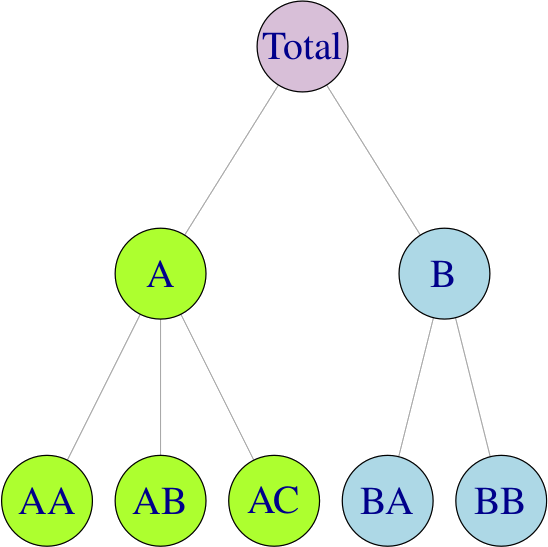
\includegraphics[scale=0.35]{figures/hts.png}
    \caption[A two-level hierarchical tree diagram]{A two-level hierarchical tree diagram \parencite{hyndman2018}.}
    \label{fig:hts}
\end{figure}



\subsubsection{Approaches to Hierarchical Forecasting}

When analysing hierarchical time series, concurrent analysis at several aggregation levels can balance computational efficiency with granularity \parencite{hyndman2018}.


Forecasting within a hierarchical system uses techniques to ensure that forecasts are credible and internally coherent: the aggregation of forecasts at one level should match the forecast of the level above.
The main approaches are bottom-up, top-down, and middle-out \parencite{hyndman2018}.

The bottom-up approach begins its predictions at the base level and aggregates them to higher levels.
This approach is computationally practical and often performs well when upper-level series are relatively stable.
The top-down approach starts at the top of the hierarchy and distributes forecasted totals using historical proportions.
The middle-out approach connects bottom-up and top-down methods by focusing on a mid-level, aiming to balance the strengths of both.

\subsection{Grouped Time Series}

Grouped time series represent collections of temporally structured data organised by shared attributes (e.g., device type, customer demographics) rather than by a single nested hierarchy.
Unlike hierarchical series, grouped data lack inherent aggregation constraints: forecasts for individual series may be developed independently and then analysed collectively for cross-sectional patterns \parencite{hyndman2018}.
Grouped time series are widely used in macroeconomic analysis \parencite{athanasopoulos2017} and supply-chain forecasting \parencite{wickramasuriya2015}, where multiple cross-sectional dimensions demand coherent alignment without a strict hierarchical dependence.

Often, disaggregating factors are both nested and crossed.
For example, Australian tourism data can be disaggregated by hierarchical geographical categories (states, and regions nested within states), but also by four purposes of travel: holiday, business, visiting friends and relatives, and other.
This grouping variable does not nest within any of the geographical variables.
\begin{figure}[H]
    \centering
    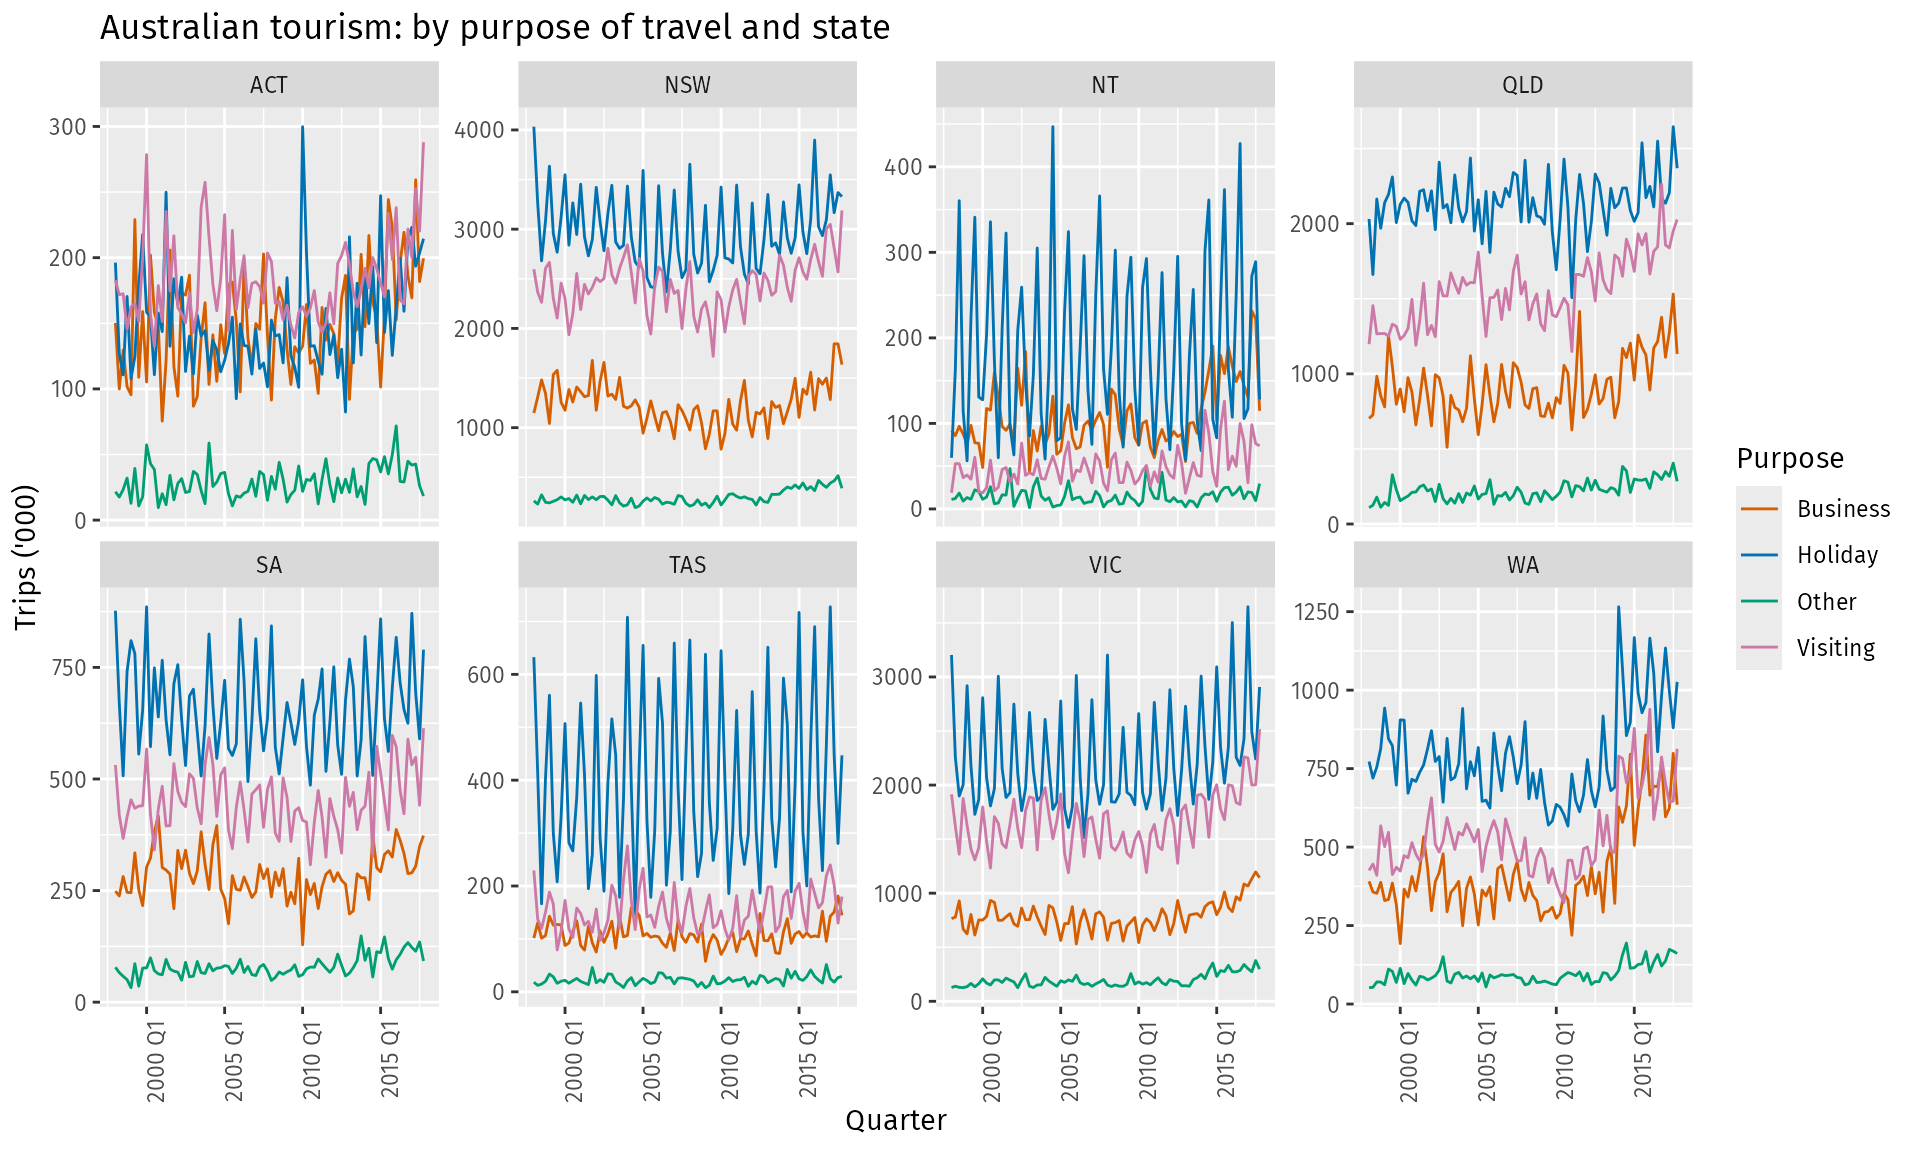
\includegraphics[scale=0.5]{figures/mixed-state-purpose.png}
    \caption[Australian domestic overnight trips, 1998 Q1--2017 Q4, by purpose and state]{Australian domestic overnight trips over the period 1998\,Q1 to 2017\,Q4 disaggregated by purpose of travel and by state \parencite{hyndman2021}.}
    \label{fig:grouped}
\end{figure}

\section{Anomaly Detection}

In machine learning, anomaly detection aims to find patterns that deviate significantly from expected behaviour \parencite{chandola2009}.
It is essential in many fields, including fault diagnosis, network security, and fraud detection.
Univariate anomaly detection identifies outliers in a single variable.
Multivariate anomaly detection considers several variables jointly, so that a point may be anomalous because of an unusual combination of values even when each variable looks normal in isolation.

Anomalies are often classified as point anomalies (a single observation is unusual), collective anomalies (a contiguous subsequence is unusual as a group), or contextual anomalies (an observation is unusual only in a given context) \parencite{chandola2009}.

\subsection{Matrix Profile and Discords}

The Matrix Profile (\ac{MP}) is introduced here because Grammatical Evolution generates many aggregations, and for each produced candidate series a scorer is needed.
\ac{MP} is exact, label-light, and computationally feasible for many candidates.
It takes one candidate time series and computes the nearest-neighbour distance for each subsequence of fixed length, then returns a discord score.

Distance is typically the z-normalised Euclidean distance between two subsequences \parencite{yeh2017timeseriesjoins}: each window is first standardised to zero mean and unit variance, so the comparison is based on shape rather than on the raw level of the series.

A time-series discord is the subsequence most distant from its nearest non-self match \parencite{keogh2005hotsax}.
On the Matrix Profile, the discord is the position with the maximum nearest-neighbour distance \parencite{yeh2017timeseriesjoins}.
For a short and unusual subsequence or spike, the discord may capture well, but may poorly capture a level shift, which is a sustained change to a new level; a ramp, which gradually drifts upwards over time; or a multivariate contextual anomaly, where each series looks normal alone but the relationship is abnormal.

\section{Anomaly Generation}

Anomaly generation is the methodical production of irregular patterns or outliers that depart significantly from normal data distributions \parencite{hawkins1980}.
In machine learning settings it is used both to stress-test system robustness \parencite{chandola2009} and to augment training or evaluation data.
Modern practice emphasises generating semantically plausible contextual anomalies for the target domain \parencite{ruff2021}.

\subsection{Rule-Based Approaches}

Expert-defined constraints in domain-specific anomaly generation deliberately break normal system behaviour \parencite{chandola2009}.
In this dissertation, synthetic anomalies are injected with rule-based thresholds (e.g., values outside $\mu \pm 3\sigma$ over a 168-hour window).

\subsection{Validation of Synthetic Anomalies}

To ensure synthetic anomalies are useful for evaluation, validation typically combines domain checks (e.g., expert judgement that injected patterns are realistic) with quantitative detection benchmarks \parencite{ruff2021}.
In this work, injected labels enable \ac{AUC} evaluation of Matrix Profile discord scores on each candidate aggregation.

\section{Grammatical Evolution}

\subsection{Combinatorial Optimization}

Combinatorial optimisation identifies optimal configurations within finite discrete solution spaces and provides formal frameworks for many NP-hard problems \parencite{papadimitriou1982,garey1979}.
Exact methods (e.g., integer programming, branch-and-bound, dynamic programming) guarantee optimality but can be computationally costly at scale \parencite{papadimitriou1998}.
Approximation and metaheuristic methods---including greedy search, local search, simulated annealing, and genetic algorithms---trade guarantees for tractable near-optimal solutions on large instances \parencite{vazirani2001,glover1989,zlochin2004}.

\subsection{Genetic Programming}

Genetic algorithms evolve a population of candidate solutions by selection, crossover, and mutation.
Genetic programming (\ac{GP}) is a specialised form of genetic algorithm that evolves computer programmes, typically represented as trees whose nodes are functions or terminals \parencite{koza1992}.
An operator of selection uses fitness to choose parents; crossover mixes elements of different parent solutions to produce offspring; mutation introduces random variation; and a survival or replacement operator forms the next generation until a stopping criterion is met.

\begin{figure}[H]
    \centering
    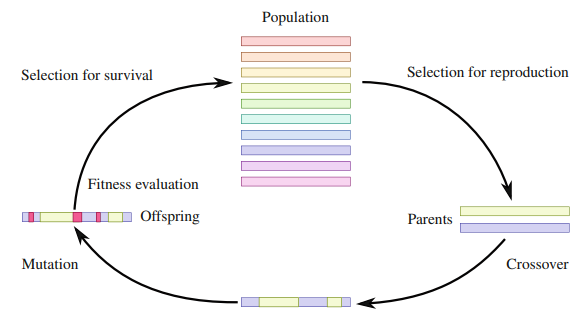
\includegraphics[scale=0.5]{figures/GP_cicle.png}
    \caption[Generational loop in an evolutionary algorithm]{Generational loop in an evolutionary algorithm.
    From a population of solutions, individuals are selected to reproduce by crossover and mutation; offspring are evaluated and incorporated; and a survival operator restores the population size.
    Source: adapted from standard evolutionary-algorithm schematics (see also \textcite{koza1992}).}
    \label{fig:generational_loop}
\end{figure}

\ac{GP} is particularly effective for symbolic regression, automated algorithm discovery, and optimisation tasks \parencite{koza1992,banzhaf2004}.
Population size and the number of generations are crucial parameters that influence exploration of the search space and convergence speed.

\subsubsection{Grammatical Evolution}

Grammatical Evolution (\ac{GE}) is a way to apply evolutionary computing to problems defined by a formal grammar \parencite{oneill2001grammatical,oneill2003}.
A formal grammar is a set of rules that define a language's syntax and allow generation of valid strings or structures.
In \ac{GE}, the genotype is an integer vector rather than a tree; the grammar maps those vectors to valid phenotypes.
This representation supports flexible adaptation to different grammar structures.

The process of Grammatical Evolution involves the following steps:
\begin{enumerate}
    \item Define a \ac{BNF} representation of the grammar;
    \item Randomly generate genotypes as integer vectors;
    \item Evaluate fitness by mapping genotypes to phenotypes and testing them against the fitness function;
    \item Use genetic operators such as crossover and mutation to evolve the population of genotypes;
    \item Repeat steps 3 and 4 until a satisfactory solution is found or a stopping criterion is met.
\end{enumerate}

\subsection{Backus-Naur Form}

A \ac{BNF} grammar describes the syntax of a language as a tuple of four sets:
\begin{itemize}
    \item $T$: the terminal set;
    \item $N$: the non-terminal set;
    \item $P$: the set of production rules;
    \item $S$: the start symbol (a member of $N$).
\end{itemize}

For example, consider a simple grammar for mathematical expressions with addition, subtraction, multiplication, and division, using variables $x$ and $y$:
\[
T = \{+, -, /, *, x, y\}, \qquad
N = \{\langle e \rangle, \langle o \rangle, \langle v \rangle\}.
\]
The non-terminal $\langle e \rangle$ denotes an expression, $\langle o \rangle$ an operator, and $\langle v \rangle$ a variable.
The production rules in $P$ are:
\begin{align}
\langle e \rangle &::= \langle e \rangle \langle o \rangle \langle e \rangle \mid \langle v \rangle \\
\langle o \rangle &::= + \mid - \mid / \mid * \\
\langle v \rangle &::= x \mid y
\end{align}
The pipe operator $\mid$ denotes alternatives.
The start symbol is $S = \langle e \rangle$.

Genotypes may be represented as non-negative integer arrays.
For example, consider
\[
C = [4, 15, 75, 8, 41, 12].
\]
Mapping begins from the start symbol $\langle e \rangle$.
The general rule is
\[
\text{selected\_option} = \text{gene\_value} \bmod r,
\]
where $\text{gene\_value}$ is the current integer from the genotype, $r$ is the number of production choices available for the current non-terminal, and $\text{selected\_option}$ is the (zero-based) index of the chosen production.

The first gene is 4 and $\langle e \rangle$ has two options, so $4 \bmod 2 = 0$ selects $\langle e \rangle \langle o \rangle \langle e \rangle$.
Continuing left-to-right:
\begin{enumerate}
    \item With gene 15, $15 \bmod 2 = 1$ replaces the first $\langle e \rangle$ with $\langle v \rangle$;
    \item With gene 75, $75 \bmod 2 = 1$ replaces $\langle v \rangle$ with $y$;
    \item With gene 8, $8 \bmod 4 = 0$ replaces $\langle o \rangle$ with $+$;
    \item With gene 41, $41 \bmod 2 = 1$ replaces the remaining $\langle e \rangle$ with $\langle v \rangle$;
    \item With gene 12, $12 \bmod 2 = 0$ replaces $\langle v \rangle$ with $x$.
\end{enumerate}
The final expression is $y + x$.

\subsection{Initialization Phase}

Initialisation can be performed on the genome or on the derivation tree.
To control tree depth, this work uses Position-Independent Grow (\ac{PIG}), which generates individuals that tend to fill the allowed depth range: neither systematically too deep nor too shallow.
\ac{PIG} expands non-terminals in random order rather than always expanding leftmost first, and ensures that at least one branch reaches the maximum depth.
This reduces duplicate structures and increases diversity in the initial population.

\subsection{Selection Mechanism}

The selection mechanism chooses individuals from the population to act as parents for the next generation while retaining some randomness to preserve diversity.
This work adopts tournament selection: a number of individuals are drawn at random, the best individual in each tournament is retained, and the process is repeated until the required number of parents has been selected.

\subsection{Variation Operators}

The variation operators explore the search space by modifying genetic material.
The two primary operators adopted in this work are crossover and mutation.

The crossover operator mixes parent genotypes to obtain offspring genotypes.
Variable one-point crossover, which was chosen for this work, swaps the tails of two parents after cut points selected independently in each parent; because the cut positions need not coincide, offspring genome lengths may differ from those of the parents, enabling combination of beneficial traits of different lengths.

Mutation is applied to every child after crossover, using a codon-based integer-flip method.
Here a codon is one element of the genotype vector: an integer flip replaces that codon with another random integer in the allowed codon range.
Each codon is mutated independently with probability
\begin{equation}
    P_{\text{mutation}} = \frac{1}{\text{genome\_length}}.
\end{equation}
In standard PonyGE2 practice this probability is applied over the genome (or over used codons, depending on configuration); the operator itself does not ``know'' which unused trailing genes will later be consumed by wrapping or unused material.

\subsection{Replacement Strategy}

The replacement strategy determines how new individuals enter the population.
This work uses generational replacement with elitism: the best individuals from the previous generation are retained, while the remaining positions are filled by newly generated offspring.
Elitism helps preserve high-quality solutions while the rest of the population continues to explore.

\section{Metrics}

\subsection{Precision and Recall}

In anomaly detection, precision and recall provide complementary perspectives on model performance, especially under class imbalance (e.g., rare fraud cases among many legitimate events).

\subsubsection{Precision}
\label{subsec:precision}

Precision quantifies a model's ability to minimise false-positive classifications:
\begin{equation}
    \text{Precision} = \frac{\text{TP}}{\text{TP} + \text{FP}},
\end{equation}
where $\text{TP}$ denotes true positives and $\text{FP}$ false positives.

\subsubsection{Recall}
\label{subsec:recall}

Recall evaluates how completely positive cases are identified:
\begin{equation}
    \text{Recall} = \frac{\text{TP}}{\text{TP} + \text{FN}},
\end{equation}
where $\text{FN}$ denotes false negatives.

\subsection{Trade-off and Applications}

Raising the decision threshold typically increases precision and decreases recall, and vice versa; the preferred balance is domain-specific.
High recall is paramount in medical diagnostics, where missing a true positive can be severe.
High precision is crucial in spam filtering, where false positives waste user attention.

\subsubsection{F1 Score}
\label{subsec:f1-score}

The F1 score is the harmonic mean of precision and recall:
\begin{equation}
    \text{F1} = 2 \cdot \frac{\text{Precision} \cdot \text{Recall}}{\text{Precision} + \text{Recall}}.
\end{equation}
It provides a single score when precision and recall should be balanced, but can be misleading under severe class imbalance, where \ac{AUC} or precision--recall curves may be more appropriate.

\subsection{Area Under the ROC Curve (AUC)}

The \ac{ROC} curve plots the true-positive rate against the false-positive rate across classification thresholds \parencite{hanley1982}.
The Area Under the ROC Curve (\ac{AUC}) is a common performance metric for binary classifiers under class imbalance \parencite{fawcett2006}.
It measures the classifier's capacity to discriminate between classes.

\subsubsection{Interpretation and Calculation}
\ac{AUC} values range from 0 to 1, where:
\begin{itemize}
    \item 0.5 indicates random guessing;
    \item 1 represents perfect separability;
    \item values below 0.5 suggest inverted ranking.
\end{itemize}

The Wilcoxon--Mann--Whitney statistic provides a non-parametric \ac{AUC} estimate \parencite{hanley1982}:
\begin{equation}
    \text{AUC} = \frac{\sum_{i=1}^{n_+} \sum_{j=1}^{n_-} \mathbf{1}(s_i^+ > s_j^-)}{n_+ \cdot n_-},
\end{equation}
where $n_+$ and $n_-$ denote the numbers of positive and negative instances and $s$ denotes classifier scores.

\subsubsection{Advantages and Limitations}
\ac{AUC} is robust to class imbalance and does not require a fixed threshold \parencite{bradley1997}.
However, it does not capture cost-sensitive decision contexts and can be misleading when ROC curves cross \parencite{lobo2008}.

\section{Literature Review}
\addtocontents{toc}{\protect\setcounter{tocdepth}{1}}

\subsection{Anomaly Detection in Telecommunications Networks}

Telecommunication anomaly detection is difficult because labels are scarce.
Moreover, the industry produces large amounts of data, with few viable labels that can be identified as anomalies.
Often, the problem is not detecting the anomaly but selecting which subsection of the network window to monitor.

\textcite{gonzalez2024one} apply a Dilated Convolutional Variational Autoencoder (DC-\ac{VAE}), a deep model that scores anomalies jointly across several related time series, to mobile-network counters.
They evaluate it on a fully aggregated view where labels are sparse: of 730{,}000 samples, only 9{,}000 were labeled, using a fixed set of 12 features.
Range-based F1 (range-F1) measures overlap between predicted and labeled anomaly intervals rather than isolated timestamps; they report a mean range-F1 of around 52\%, which is only modest.

\textcite{burgueno2020online} indicate that the network they analyzed had 25{,}000 mobile base station coverage areas.
Moreover, for each cell they analyzed 240 hourly \ac{KPI}s, but the study focuses on only 15 of the most important.
Detection is an online threshold state machine (normal / border / anomalous) run at cell level on that manually selected subset; they report capturing almost 80\% of the labeled network anomalies.
From this perspective, manual selection is a bottleneck because the 225 unmonitored features may still contain relevant information; for example, anomalies may occur in an unmonitored signal.

Call Detail Records (\ac{CDR}) and mobile activity records are recognized for analysis in telecom monitoring.
\textcite{sultan2018cdr} report no detection metrics.

\textcite{lemaire2024early} study early detection of urban events from Orange France mobile Network Signalling Data in Paris: cell-level, one-minute counts of network services (calls, SMS, and related signalling).
They use a Signature detector and hand-designed categorical aggregations over these service types, not temporal aggregation.
Against a curated set of documented urban events, their best precision is 28.63\%, with event recall of about 36\% at the corresponding operating point, indicating many false alarms even when the signal is useful.

Existing work assumes a fixed aggregation and therefore may miss anomalies that would only appear under a different grouping.
Automated search is useful when the best aggregation is not obvious in advance; in those papers, there is a fixed review of aggregation, but they do not address how to automate the aggregation of time series.
The next section will be about this topic.

\subsection{Anomaly Detection in Grouped Time Series}

Anomaly detection in grouped time series treats the detector input as a chosen representation, not the whole network.
The dataset is aggregated by related features/entities at the aggregation level, rather than treating a network as a flat collection of features.
It is important because the detection quality is dependent on the aggregation of features, not only the detector.
Across the reviewed studies, datasets, labels, and metrics differ, so reported scores are not directly comparable.

\textcite{mefleh2025beyond} used an unsupervised Mahalanobis distance approach in a telecommunications setting.
They report \ac{AUC} rising from 0.77 on the raw \ac{KPI} features to 0.86 when denominator information is included (for example, attempt counts that normalise ratios), then to 0.93 with adjusted ratios, and finally to 0.99 with learned adjustments.
This result shows that detection quality changes with feature transformation and aggregation.

\textcite{hua2022genad} show that China Mobile wireless base stations share some operational behavior, which GenAD, a generative reconstruction model, can learn and then use to detect anomalies on other stations in the same network.
GenAD was pre-trained on 3{,}000 unlabeled base stations, using multivariate time series features.
Their F1 score is 0.953 (precision 0.910).
That F1 uses point-adjusted segment scoring: if any timestamp inside a labeled anomaly interval is flagged, the whole interval counts as detected, so the score is not a timestamp-wise F1.

In the study by \textcite{oguz2022anomaly}, they simulate a multi-tier network that includes aggregations from the user equipment measurements and classifies the state of each femtocell access point.
Performance changes with the region of interest (\ac{ROI}) radius, signal shadowing, and aggregation methods.
At a 30\,m \ac{ROI} with 2\,dB shadowing, the 1D \ac{CNN} achieved 80.1\% accuracy, but as \ac{ROI} size and the shadowing increase, the accuracy decreases, so this shows that including more observations is not necessarily beneficial when added signals are less relevant or noisier.

Based on the reviewed studies, we can extract that grouping can strongly affect anomaly detection performance.
Although aggregations are selected manually before modeling the relevant \ac{KPI}s, entities, aggregation levels, and spatial boundaries, none of them systematically search for an aggregation structure that best characterizes the anomaly.

\subsection{Anomaly Detection in Hierarchical Time Series}

Hierarchy in anomaly detection is important because an alert such as ``traffic is abnormal'' is not enough for a telecom operator to act on.
The operator must determine whether it affects the entire network, a region or specific cell of the switch, or only one \ac{KPI} category.
So this top-down approach helps break down into smaller branches; although that hierarchy is not necessarily the best aggregation for detecting anomalies.

\textcite{hong2012tiresias} detect and localize anomalies in hierarchical \ac{ISP} call-detail data.
It analyzes customer-care call logs and signaling call records across predefined hierarchies, allowing operators to identify not only that an abnormal behavior occurs but also the level at which it appears.
They found over 94\% of reference anomalies, and separately reported 99.7\% anomaly identification accuracy.
These results were obtained from a fixed additive hierarchy and Holt--Winters spike forecasting.
So the author demonstrates hierarchical localization rather than searching over alternative aggregation structures.
It does not search for alternative partial aggregations or score non-spike discords, which is the gap addressed by this thesis.

On the other hand, \textcite{wolff2022composite} treat anomaly localization as the sequential search problem of a known tree of processes.
Instead of measuring every leaf process equally, their hierarchical dynamic search method first samples aggregate internal nodes and then moves towards the branch most likely to contain an anomaly.
This shows that hierarchy can be an active search space, not merely a reporting structure used after detection.
However, Wolff assumed tree topology is already known, as search is only within it.
This differs from our approach, which uses a \ac{GE} to generate candidate aggregations before applying the anomaly scorer.

\textcite{huang2026hydra} propose HYDRA, a multi-level hierarchy-driven anomaly detector that builds several hierarchy-based views of each series and combines detection signals across those levels.
It ranked first among 40 algorithms across 40 TSB-AD datasets.

\subsection{Matrix Profile and Time-Series Discord Detection}

Chapter~2 defined the Matrix Profile and discords.
What belongs in this chapter is the published evidence that the scorer is fast enough for many candidate series, and whether it has been used on telecommunications data.

Computational efficiency is substantially improved: a refinery time-series self-join is reduced from an estimate of 153.8 days by brute force to 1.2 hours with STAMP/STOMP \parencite{yeh2017timeseriesjoins}.
Also, \textcite{zhu2016matrixprofileii} showed GPU-STOMP could process 100 million subsequences in about 12 days, compared to the estimate of 1585 years for brute force.
STUMPY \parencite{law2019stumpy} gives the practical implementation of this process in Python.
\textcite{vanonsem2023motif} apply Matrix Profile to production \ac{KPI} series from telecom-provider customers of Skyline Communications (25 series), using it for variable-length \emph{motif} discovery rather than discord scoring.
They report the method is about 3--8 times faster than VALMOD; an example series yields both a 288-point (about one day) motif and a 12-point (about one hour) motif in a single distance-matrix pass.
No detection precision, recall, F1, or \ac{AUC} is reported (manual motif checks).
The series to analyse are chosen in advance, so the paper does not search aggregations.

\subsection{Combinatorial Optimisation for Selecting Time Series}

Little published work searches hierarchical aggregation structures.
Feature-selection methods are reviewed here instead because, from an optimisation viewpoint, the problems are similar: both search a combinatorial space of candidates and score each one with a fitness function.
The spaces themselves differ: feature selection chooses a subset of columns, whereas this dissertation searches grammar-constrained hierarchies.

For feature selection, $n$ features give $2^n$ candidate subsets, so exhaustive search is infeasible for large $n$; \textcite{xue2016survey} survey the evolutionary algorithms used for this search, including genetic algorithms, genetic programming, particle swarm optimisation, ant colony optimisation and differential evolution.

\textcite{linares2024evolutionary} use a genetic algorithm (SEISEN) whose fitness is a filter score, the Conditional Dependence Coefficient, to select lagged features for a multilayer perceptron forecaster.
On an electricity dataset, the feature set falls from 7{,}704 to 3{,}813 while \ac{MAE} improves from 207.193 to 194.400, showing that pruning the input representation can improve accuracy.

\textcite{pietron2025adnev} apply a genetic algorithm at three levels to multivariate time-series anomaly detection: it evolves subsets of input series, an autoencoder architecture for each subset, and the network weights, using validation loss as fitness.
On four sensor benchmarks (SWaT, WADI, MSL and SMAP), the resulting ensemble achieves the best point-wise F1 of 14 methods, with a mean of 0.70 against 0.54 for the next best, at a cost of up to 132 GPU-hours per dataset.

\textcite{he2021mining} search subspaces of high-dimensional financial transaction series with a greedy heuristic and an evolutionary $(\mu+\lambda)$ algorithm, scoring each candidate by discord mining.
On real data, greedy search achieves the higher mean average precision (0.86 against 0.72) but is about 15 times slower (1{,}345\,s against 88\,s).

Across these studies, the common pattern is an evolutionary search over a large candidate space with a fitness function evaluated per candidate.
None searches hierarchical aggregation structures, and none combines the search with a Matrix Profile scorer on telecommunications data; this dissertation does both with grammatical evolution.
\addtocontents{toc}{\protect\setcounter{tocdepth}{1}}


\chapter{Materials and Methodology}
\label{chap:methodology}

This chapter describes the data, the method and its implementation.
Section~\ref{sec:problem-formulation} presents the telecommunications dataset, analyses its categorical features and states the problem formally.
Section~\ref{sec:adopted-methodology} gives an overview of the pipeline.
The following sections describe each stage in detail: the injection of synthetic anomalies (Section~\ref{sec:anomaly-injection}), the representation of candidate hierarchies with a grammar (Section~\ref{sec:hierarchies}), the fitness function that scores a hierarchy with the \ac{MP} and the \ac{AUC} (Section~\ref{sec:fitness-evaluation}), and the configuration of the \ac{GE} search (Section~\ref{sec:ge-implementation}).
Section~\ref{sec:tools} closes the chapter with the software tools and the computational environment.

\section{Problem Formulation}
\label{sec:problem-formulation}

This research develops a hierarchical anomaly detection framework for mobile network data, with the aim of improving service reliability.
Its central question is at which level of aggregation the traffic should be monitored: a single fully aggregated series hides anomalies that affect a small segment of the traffic, while one series per combination of categorical values produces too many sparse series to monitor and interpret.
The framework answers this question with a search: candidate aggregation hierarchies are generated by a grammar, evolved with \ac{GE}, and ranked by how well a label-free detector finds known anomalies in the series they produce.

\subsection{Data Description}

The data comes from a network switch of a mobile operator and covers July to October 2022.
Each record counts the call events of one combination of categorical values in one hour, and corresponds to an aggregate of \ac{CDR}s.
The raw extract is a semicolon-separated file in which date and hour are stored in separate columns.
During preparation the two are combined into one hourly timestamp, the \#Events column is cleaned of non-numeric characters and converted to integers, the columns not used in this work (data source, date, hour and Event Duration) are dropped, and duplicated records are removed.
The resulting working dataset of 958{,}479 hourly records, spanning 2{,}110 hours from 18 July to 13 October 2022, is used throughout this dissertation.

The switch reports two metrics: \#Events, the number of call events, and Event Duration, the total call time.
Only \#Events is used as the target variable in this work, because event counts are available for both voice and SMS traffic and are the usual indicator of traffic volume.
Each record is described by six categorical features, listed in Table~\ref{tab:cdr_fields}.

\begin{table}[H]
    \centering
    \caption[Categorical features of the switch records]{Categorical features of the switch records. The letter is the symbol used for the feature in the grammar (Section~\ref{sec:grammar}).}
    \label{tab:cdr_fields}
    \begin{tabularx}{\textwidth}{llX}
        \toprule
        Letter & Feature & Description and values \\
        \midrule
        A & Call Type & Type of communication: SMS, VOICE. \\
        B & Event Type & Role of the event in the call: ORIGINATED, CALL FORWARD, TERMINATED, ROAMING OUT. \\
        C & Subscriber Type & Type of subscriber: Postpaid, Application, Roamer In, Prepaid, Other. \\
        D & Traffic Type & Destination of the traffic: OFF-NET (another operator), INT (international), ON-NET (same operator). \\
        E & Service Type & Whether the subscriber is roaming: NOT-ROAMING, ROAMING. \\
        F & Partner Description & Anonymised partner operator associated with the traffic: 392 values, P\_0001 to P\_0392. \\
        \bottomrule
    \end{tabularx}
\end{table}

Figure~\ref{fig:telecom_groups} shows the fully aggregated traffic over the whole period and Figure~\ref{fig:daily_events} zooms into eleven days of \#Events.
Both show a strong daily cycle, with low traffic at night and peaks during the day, and a weekly pattern in which weekend days differ from working days.
This regularity is what makes a shape-based detector suitable: an anomaly appears as an hour that breaks the expected daily and weekly shape.
It also motivates the window of about one week used both to inject anomalies (Section~\ref{sec:anomaly-injection}) and to compute the \ac{MP} (Section~\ref{sec:fitness-evaluation}), since one week is the shortest window that contains a complete cycle of both patterns.

\begin{figure}[H]
    \centering
    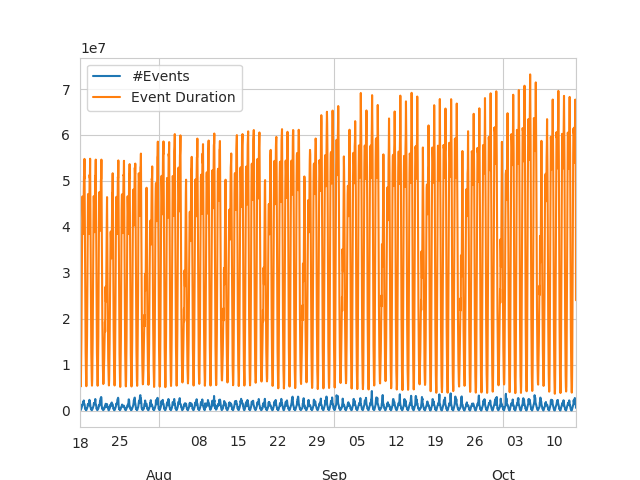
\includegraphics[scale=0.35]{figures/telecom_traffic_hierarchy.png}
    \caption[Telco network traffic metrics (\#Events and Event Duration) over July-October 2022 aggregated.]{Hourly network traffic patterns showing (A) Total \#Events (left axis) and Event Duration in hours (right axis).}
    \label{fig:telecom_groups}
\end{figure}

\begin{figure}[H]
    \centering
    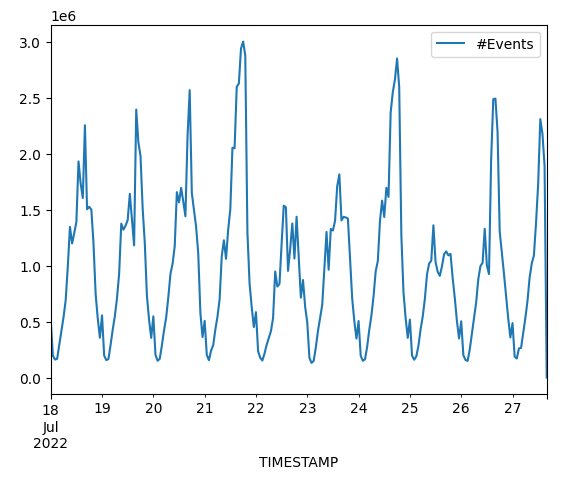
\includegraphics[scale=0.35]{figures/event_count_trend.png}
    \caption[Daily \#Events from 18--28 July 2022]{Hourly call event frequency.}
    \label{fig:daily_events}
\end{figure}

\subsection{Categorical Feature Analysis}

The six features can in theory be combined into $2 \times 4 \times 5 \times 3 \times 2 \times 392 = 94{,}080$ distinct combinations, but only 1{,}555 of them occur in the data.
Each non-empty combination is observed on average in 614 of the 2{,}110 hours of the period, with a median of only 182 hours: 94 combinations are present in every hour, while 127 appear in a single hour, so most of the corresponding series are zero for most of the time.
Table~\ref{tab:categorical_dist} describes each feature over these 1{,}555 combinations, and adds the share of the total \#Events carried by the most frequent category.

\begin{table}[H]
    \centering
    \caption[Cardinality and Dominant Categories in Telco Data]{Cardinality and Dominant Categories in Telco Data. Unique Values is the number of categories per variable; Frequency counts are out of the 1,555 non-empty feature combinations, not out of records. The last column is the share of all \#Events carried by the same top category.}
    \small
    \begin{tabular}{lrlrr}
        \toprule
        Variable & Unique Values & Top Category & Frequency & Share of \#Events \\
        \midrule
        Call Type & 2 & VOICE & 849 (54.6\%) & 45.2\% \\
        Event Type & 4 & ORIGINATED & 716 (46.0\%) & 18.3\% \\
        Subscriber Type & 5 & Roamer In & 1,486 (95.6\%) & 5.7\% \\
        Traffic Type & 3 & INT & 1,486 (95.6\%) & 21.8\% \\
        Service Type & 2 & NOT-ROAMING & 1,544 (99.3\%) & 92.4\% \\
        Partner Description & 392 & P\_0001 & 65 (4.2\%) & 94.3\% \\
        \bottomrule
    \end{tabular}
    \label{tab:categorical_dist}
\end{table}

The table reveals three distribution patterns:
\begin{itemize}
    \item \textbf{Highly skewed features.} Subscriber Type, Traffic Type and Service Type are dominated by one category in terms of combinations: 95.6\% of the combinations are Roamer In and international (INT) traffic, and 99.3\% are not roaming. Inbound roamers are associated with many different partner operators, so they generate most of the distinct combinations.
    \item \textbf{Balanced features.} Call Type (54.6\% VOICE, 45.4\% SMS) and Event Type (46.0\% ORIGINATED) split the combinations more evenly.
    \item \textbf{High-cardinality feature.} Partner Description has 392 values with a long-tail distribution; the most frequent partner appears in only 4.2\% of the combinations.
\end{itemize}

Counting combinations and counting traffic give very different pictures.
Roamer In accounts for 95.6\% of the combinations but only 5.7\% of the events: most of the traffic comes from Prepaid subscribers (63.3\% of all \#Events) and stays inside the operator's network (ON-NET, 61.3\%).
Conversely, partner P\_0001 appears in only 4.2\% of the combinations but carries 94.3\% of the events.
In other words, a few combinations carry most of the traffic, while most combinations are small and sparse.
This matters for the method: a leaf of a hierarchy that isolates a high-volume segment produces a dense, regular series, whereas a leaf that isolates a rare combination produces a sparse series that is hard to score (Section~\ref{sec:fitness-evaluation}).

The information content of each feature is measured with the Shannon entropy of its distribution over the combinations,
\begin{equation}
    H = -\sum_{i=1}^{n} p_i \log_2 p_i,
\end{equation}
where $p_i$ is the proportion of combinations with category $i$ and $n$ the number of categories.
The entropy is 0 bits when a feature takes a single value and reaches $\log_2 n$ when all values are equally frequent.
Table~\ref{tab:entropy} lists the values.

\begin{table}[H]
    \centering
    \caption[Information content by variable]{Information content by variable, computed over the 1,555 non-empty combinations. The maximum is the entropy of a uniform distribution over the same number of categories.}
    \label{tab:entropy}
    \begin{tabular}{lrr}
        \toprule
        Variable & Entropy (bits) & Maximum $\log_2 n$ (bits) \\
        \midrule
        Call Type & 0.994 & 1.000 \\
        Event Type & 1.361 & 2.000 \\
        Subscriber Type & 0.349 & 2.322 \\
        Traffic Type & 0.306 & 1.585 \\
        Service Type & 0.061 & 1.000 \\
        Partner Description & 8.404 & 8.615 \\
        \bottomrule
    \end{tabular}
\end{table}

Partner Description has by far the highest entropy (8.4 bits, close to its maximum), so splitting on it creates hundreds of branches, most of them containing very little traffic.
This has two consequences.
First, its 392 values would make the grammar and the search space much larger: every split on Partner Description would create 392 child nodes.
Second, the resulting leaves would be the sparse series on which the detector performs worst.
Partner Description is therefore excluded from the search space.
It is present in the data and in the full grammar \texttt{grammars/mobai.pybnf} (letter F), but it is dropped from \texttt{grammars/mobai\_nop.pybnf}, the grammar used in the experimental campaign.
Without it, only 77 of the $2 \times 4 \times 5 \times 3 \times 2 = 240$ possible combinations of the remaining five features occur in the data.
At the other extreme, Service Type has almost no entropy (0.06 bits): nearly all combinations are not roaming, so a split on it produces one large branch and one very small one.
It is kept in the grammar, and the search decides whether such a split is useful.

\subsection{Formal Problem Statement}
\label{sec:problem-statement}

Let each record $r$ have values $x_1(r), \dots, x_5(r)$ for the five features A--E, an hour $t(r)$, an event count $e(r)$ and an anomaly flag $a(r) \in \{0,1\}$ (Section~\ref{sec:anomaly-injection}).
A \emph{filter} $\phi$ is a conjunction of conditions of the form $x_j = v$, with at most one condition per feature, for example $\phi = (\text{Event Type} = \text{ORIGINATED}) \land (\text{Call Type} = \text{SMS})$.
Each filter defines an hourly series and its labels:
\begin{equation}
    s_\phi(t) = \sum_{r \,:\, \phi(r),\; t(r) = t} e(r),
    \qquad
    y_\phi(t) = \max_{r \,:\, \phi(r),\; t(r) = t} a(r),
    \label{eq:leaf-series}
\end{equation}
so $s_\phi(t)$ is the number of events of the matching records at hour $t$, and hour $t$ is anomalous in this series if any of these records was modified by the injection.
Hours without matching records have $s_\phi(t) = 0$ and $y_\phi(t) = 0$.

A \emph{hierarchy} $H$ is a tree whose root represents all traffic.
Each internal node splits its traffic on one feature not yet used on the path from the root, creating one child per value of that feature; each leaf $\ell$ therefore corresponds to the filter $\phi_\ell$ formed by the conditions on its path.
Because every split covers all values of the feature, the leaves of a hierarchy partition the records: each record belongs to exactly one leaf, so no traffic is lost or counted twice.
The fully aggregated series is the hierarchy with a single leaf and an empty filter.

Let $\mathcal{L}(G)$ be the set of hierarchies generated by the grammar $G$ (Section~\ref{sec:hierarchies}) and $F(H; D)$ the fitness of hierarchy $H$ on the data $D$, defined in Section~\ref{sec:fitness-evaluation}.
The problem is to find
\begin{equation}
    H^{*} = \arg\max_{H \in \mathcal{L}(G)} F(H; D_{\text{train}}),
    \label{eq:problem}
\end{equation}
the hierarchy whose leaf series allow a fixed, label-free detector to separate the injected anomalies from normal hours as well as possible on the training period.
The hierarchy found is then evaluated, without further changes, on the test period $D_{\text{test}}$.

\section{Adopted Methodology}
\label{sec:adopted-methodology}

Figure~\ref{fig:workflow} summarises the pipeline, which has five stages.

\begin{figure}[H]
    \centering
    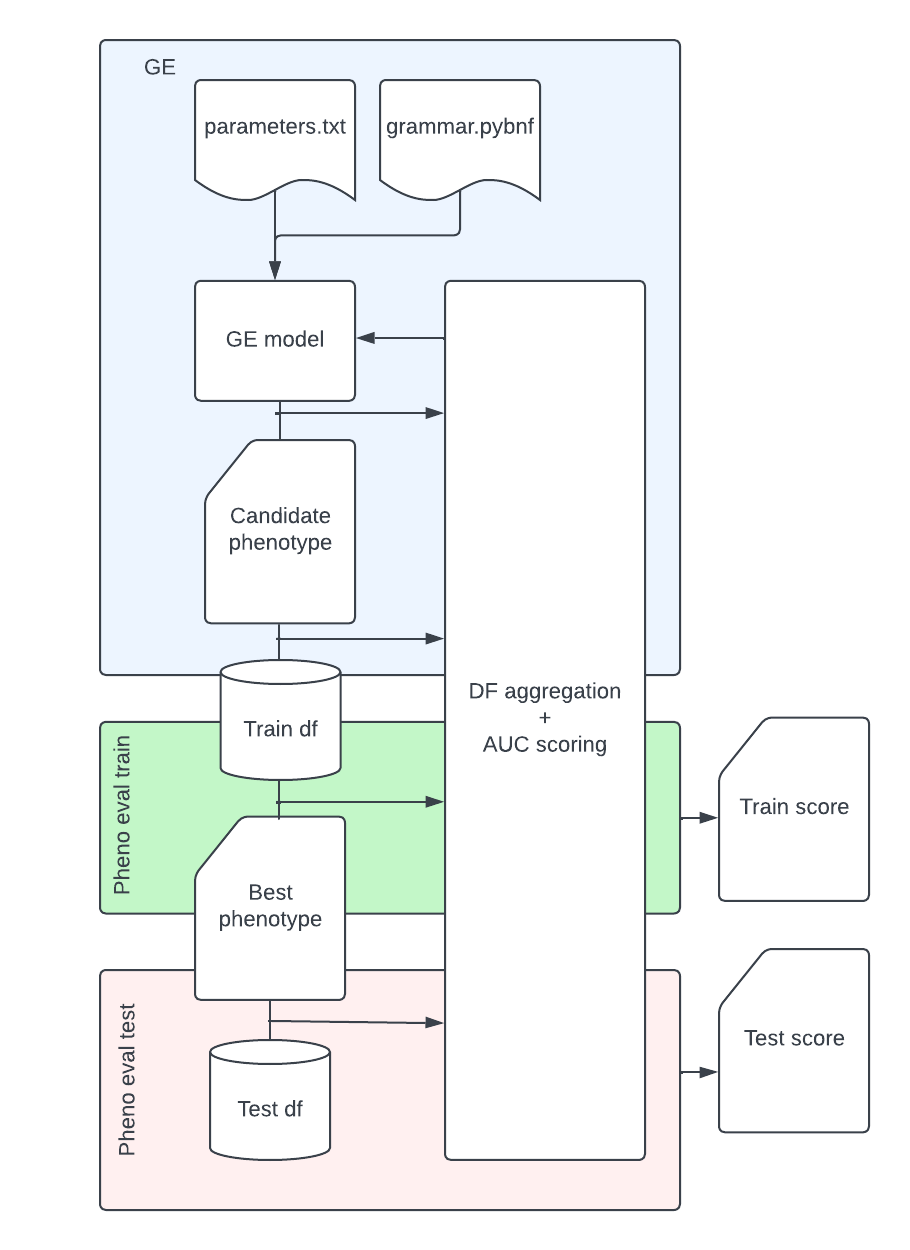
\includegraphics[scale=0.35]{figures/workflow_diagram.png}
    \caption[Anomaly detection workflow]{Hierarchical anomaly detection pipeline combining data aggregation, synthetic anomaly injection, and genetic model optimization.}
    \label{fig:workflow}
\end{figure}

\begin{enumerate}
    \item \textbf{Data preparation.}
    The raw extract is cleaned, the unused columns are dropped and duplicated records are removed, leaving 958{,}479 hourly records with six categorical features and the \#Events count.
    The records are kept disaggregated: series are built later, separately for each hierarchy, because each hierarchy defines its own aggregation.

    \item \textbf{Anomaly injection.}
    The operational data has no reliable anomaly labels, so synthetic point anomalies are inserted into 105 randomly chosen (combination, hour) pairs, one for about 5\% of the 2{,}110 hours, and the modified records are flagged (Section~\ref{sec:anomaly-injection}).
    These flags are the ground truth for the evaluation; the detector itself never sees them.

    \item \textbf{Data partitioning.}
    The data is split temporally, without shuffling, so that the test period lies entirely after the training period, as it would in operation.
    The training period runs from 18 July to 14 September 2022 (1{,}411 hours, 630{,}861 records) and the test period from 14 September to 13 October 2022 (699 hours, 327{,}618 records), roughly two thirds and one third of the data.
    The training period contains 75 anomalous hours and the test period 28.

    \item \textbf{Hierarchy search.}
    PonyGE2 evolves a population of candidate hierarchies generated by the grammar \texttt{mobai\_nop.pybnf} (Sections~\ref{sec:hierarchies} and~\ref{sec:ge-implementation}).
    Each candidate is evaluated on the training period only: its leaf series are built with Equation~\eqref{eq:leaf-series}, scored with the \ac{MP}, and compared with the anomaly flags through the weighted \ac{AUC} (Section~\ref{sec:fitness-evaluation}).

    \item \textbf{Evaluation.}
    The best hierarchy of each run is re-evaluated on the training and test periods and compared with fixed aggregation baselines (Chapter~\ref{chap:results}).
\end{enumerate}

The detector is the same in every case.
What changes from one candidate to another is only the set of series it is applied to, so differences in fitness measure the effect of the aggregation and not of the detector.

\section{Anomaly Injection}
\label{sec:anomaly-injection}

Since the operational dataset does not contain reliable anomaly labels, synthetic anomalies are injected to create a labelled evaluation scenario.
Injection has two advantages over expert labels: the position of every anomaly is known exactly, and anomalies can be placed at every level of aggregation, from the whole network to a single combination of categories.
The procedure is shown in Figures~\ref{fig:anomaly_workflow} and~\ref{alg:injection}.

\begin{figure}[htbp]
    \centering
    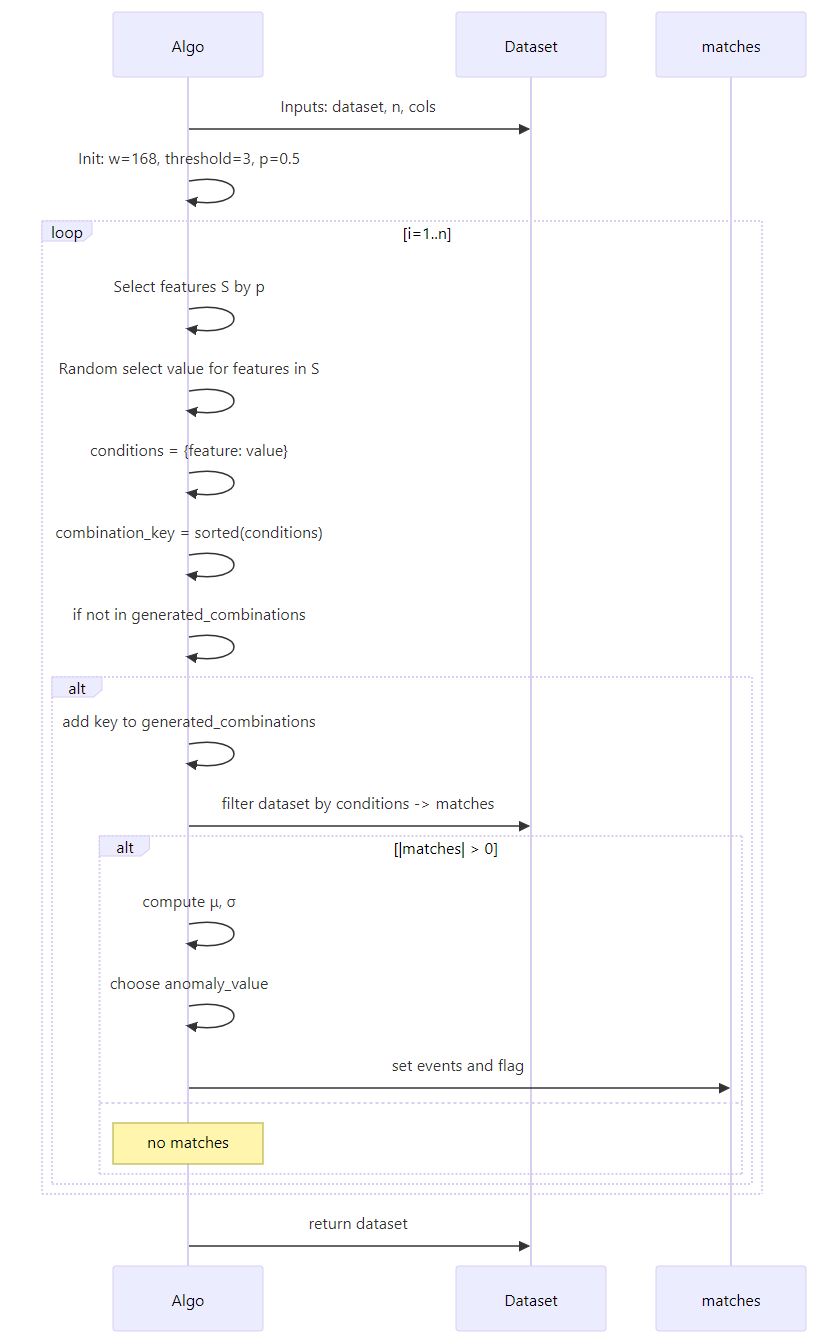
\includegraphics[height=0.75\textheight]{figures/Anomaly insertion workflow.png}
    \caption[Anomaly injection cycle]{Anomaly injection cycle.}
    \label{fig:anomaly_workflow}
\end{figure}

Each anomaly is created in four steps.
\begin{enumerate}
    \item \textbf{Choice of the affected segment.}
    Each of the six categorical features is selected independently with probability 0.5, and a value is drawn at random for each selected feature, for example $\{\text{Service Type} = \text{ROAMING}, \text{Traffic Type} = \text{INT}\}$.
    The number of conditions therefore varies: few conditions give a broad segment, such as all international traffic, and many conditions a narrow one, such as one partner for one subscriber type.
    If no feature is selected the anomaly affects all traffic.
    A combination that was already used, or that matches no records, is discarded and a new one is drawn.
    All six features are eligible, including Partner Description, so some anomalies affect segments that the grammar cannot isolate.

    \item \textbf{Choice of the hour.}
    An hour $t^{*}$ is drawn uniformly among the hours in which the segment has records.

    \item \textbf{Reference distribution.}
    The hourly \#Events series of the segment is built over the hours in which it has records, and its mean $\mu$ and standard deviation $\sigma$ are computed over a window of 167 observations around $t^{*}$ (the 84 before it, $t^{*}$ itself and the 82 after it, truncated at the ends of the series).
    For a segment present in every hour this window covers one week minus one hour and therefore a complete daily and weekly cycle; for a sparse segment, which has no records in some hours, the same number of observations spans a longer period.
    If the segment has a single observation, no window can be formed and the value is instead halved or increased by half, with equal probability.

    \item \textbf{Modification.}
    With equal probability, the anomaly is a peak or a drop.
    The new value of the segment at $t^{*}$ is $v^{*} = \mu + 3\sigma$ for a peak and $v^{*} = \max(\mu - 3\sigma, 0)$ for a drop, since an event count cannot be negative.
    The records of the segment at $t^{*}$ are rescaled by the same factor $v^{*}/s(t^{*})$, where $s(t^{*})$ is their original total, so the anomaly is distributed over the records in proportion to their original values; the new counts are rounded to integers and the records are flagged as anomalous.
\end{enumerate}

\begin{figure}[H]
    \centering
    \begin{minipage}{0.92\textwidth}
    \begin{algorithmic}[1]
        \Require records $D$, features $X_1,\dots,X_6$, number of anomalies $n$, window $w = 167$, $k = 3$
        \State $U \gets \emptyset$ \Comment{combinations already used}
        \While{fewer than $n$ anomalies have been inserted}
            \State $S \gets \{X_j : \text{a uniform random number} < 0.5\}$
            \State $\phi \gets \bigwedge_{X_j \in S} (X_j = v_j)$, with each $v_j$ drawn from the values of $X_j$
            \If{$\phi \in U$ \textbf{or} no record matches $\phi$} \textbf{continue} \EndIf
            \State $U \gets U \cup \{\phi\}$
            \State $t^{*} \gets$ hour drawn uniformly among the hours with records matching $\phi$
            \State $\mu, \sigma \gets$ mean and standard deviation of $s_\phi$ over the $w$ observations around $t^{*}$
            \State $v^{*} \gets \mu + k\sigma$ or $\max(\mu - k\sigma, 0)$, each with probability 0.5
            \For{each record $r$ with $\phi(r)$ and $t(r) = t^{*}$}
                \State $e(r) \gets \mathrm{round}\big(e(r) \cdot v^{*} / s_\phi(t^{*})\big)$; \quad $a(r) \gets 1$
            \EndFor
        \EndWhile
        \State \Return $D$
    \end{algorithmic}
    \end{minipage}
    \caption[Anomaly injection procedure]{Anomaly injection procedure.}
    \label{alg:injection}
\end{figure}

Figure~\ref{fig:anomaly_log} shows part of the log produced by the procedure.
In the first row the segment is all international traffic (Traffic Type = INT) at 08:00 on 10 September 2022: with $\mu = 234{,}009$ and $\sigma = 119{,}169$, the peak value is $\mu + 3\sigma = 591{,}516$, against an actual value of 261{,}851, so every matching record is multiplied by about 2.26.
Most of the other rows shown are drops.
For hourly traffic $\sigma$ is large relative to $\mu$, because the daily cycle alternates busy and quiet hours, so $\mu - 3\sigma$ is negative and every drop sets the segment to zero.
Drops therefore behave like outages of the segment: 30 of the 75 anomalous hours in the training period and 12 of the 28 in the test period are drops to zero, and the rest are peaks.
The 105 anomalies fall on 103 distinct hours, because in two cases the hour drawn for a new segment had already received an anomaly on another segment.

The procedure was implemented in a Kaggle notebook and executed once, without a fixed random seed.
Its output, the full record table with the modified counts and the anomaly flags, was saved and then split into the training and test sets, which are used unchanged in every run and in the final evaluation; the injected anomalies are therefore identical across all experiments, even though a new execution of the procedure would draw different ones.

\begin{figure}[htbp]
    \centering
    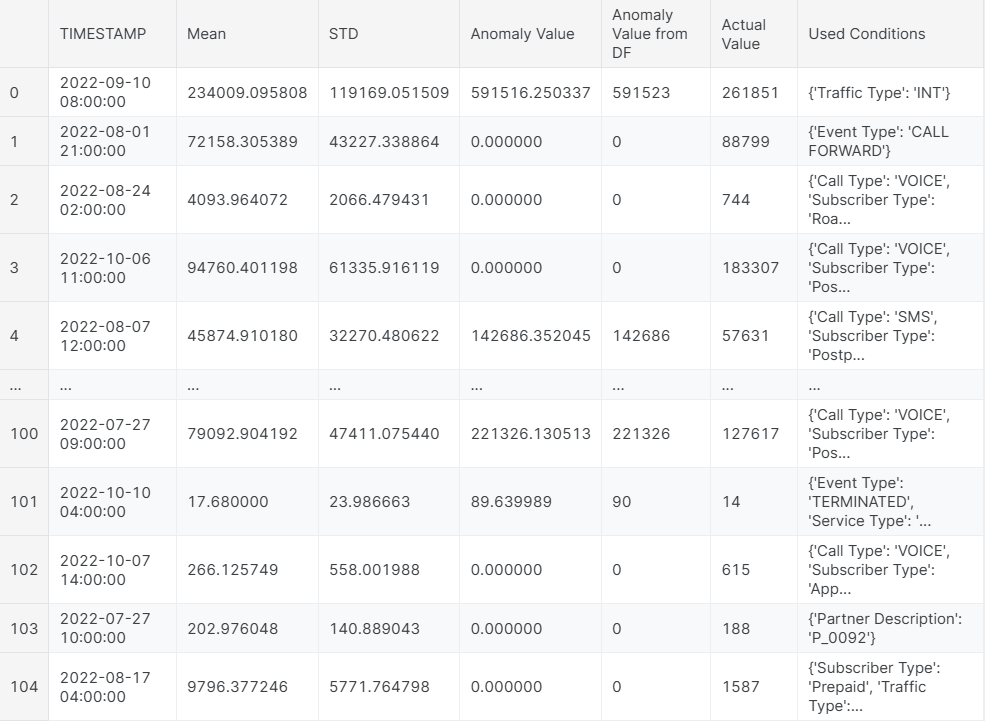
\includegraphics[width=0.95\textwidth]{figures/Anomaly log.png}
    \caption[Log of the injected anomalies]{Part of the log of injected anomalies: hour, mean and standard deviation of the segment over the reference window, target value $v^{*}$, value obtained after rounding, original value and conditions that define the segment.}
    \label{fig:anomaly_log}
\end{figure}

The window of about one week only defines the reference distribution: each anomaly is a \emph{point} anomaly that affects one hour of one segment, and the rest of the series is unchanged.
An anomaly is extreme relative to \emph{its own} segment, but it is diluted in any series that also contains other traffic.
Figure~\ref{fig:anomaly_plot} illustrates this with the two anomalies discussed above.
The peak on international traffic more than doubles that segment, but in the total traffic, of which INT is only about a fifth, the same hour lies well inside the daily range.
The drop sets CALL FORWARD events to zero, a clear outage of that segment, while the total traffic at that hour looks like an ordinary evening value.
An anomaly is easiest to detect in a series that is close to its segment, which is precisely why the choice of aggregation matters and why it is the object of the search.
Conversely, in a series that is much narrower than its segment the anomaly is spread over several leaves, each receiving the same relative change.

\begin{figure}[htbp]
    \centering
    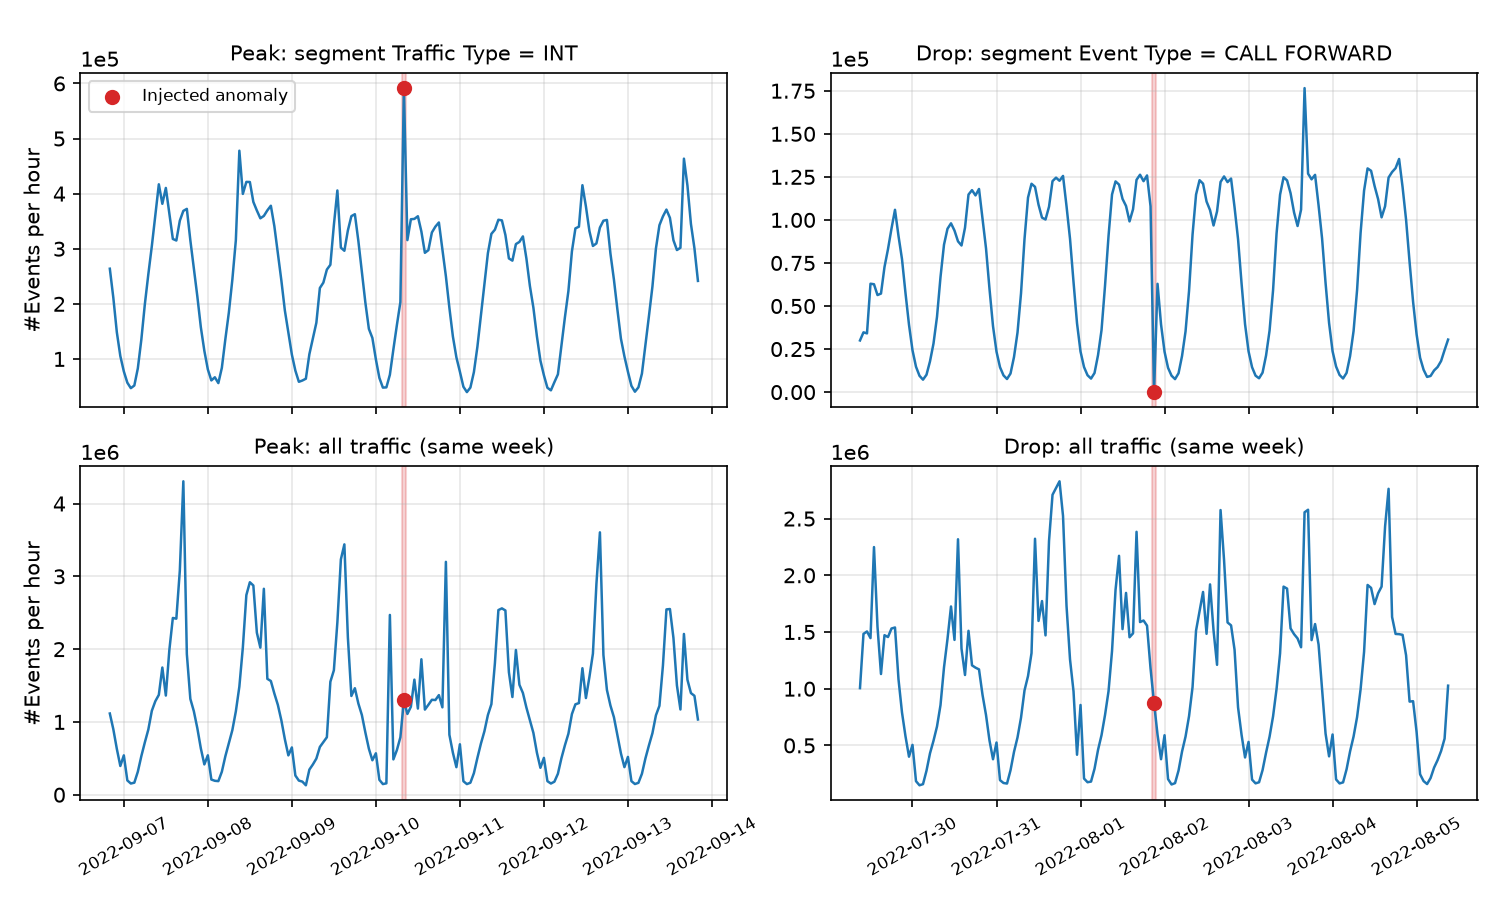
\includegraphics[width=\textwidth]{figures/injection_example.png}
    \caption[Injected anomalies on their segment and on the total traffic]{Two injected anomalies, a peak (left) and a drop (right), shown over one week on the segment that received them (top) and on the fully aggregated series (bottom). The anomalous hour is marked in red.}
    \label{fig:anomaly_plot}
\end{figure}

\section{Hierarchical Data Structures}
\label{sec:hierarchies}

There is no unique way to aggregate the data.
The same records can be monitored as one total series, as one series per call type, as one series per combination of call type and subscriber type, or by any mixture in which different branches are split on different features.
This section describes how the space of admissible hierarchies is defined with a grammar and how a hierarchy is turned into the set of series that are scored.

\subsection{Size of the Search Space}

Let $T(S)$ be the number of distinct hierarchies that can be built below a node when the features in $S$ are still unused on its path.
The node is either a leaf, or it splits on some feature $f \in S$ into $k_f$ children, each of which is again an arbitrary hierarchy over $S \setminus \{f\}$:
\begin{equation}
    T(\emptyset) = 1,
    \qquad
    T(S) = 1 + \sum_{f \in S} T(S \setminus \{f\})^{k_f}.
\end{equation}
With the five features A--E and $k_f = 2, 4, 5, 3, 2$ values, $T(\{A,\dots,E\}) \approx 2.2 \times 10^{61}$.
Exhaustive evaluation is therefore impossible, even though each hierarchy has at most 240 leaves, and the hierarchy must be found by a heuristic search.
The number of hierarchies grows so quickly because the branches of a node are independent: the traffic of one call type may be split by subscriber type while the traffic of the other call type is not split at all.

\subsection{Grammar}
\label{sec:grammar}

The admissible hierarchies are defined by the \ac{BNF} grammar \texttt{grammars/mobai\_nop.pybnf}, which has a single non-terminal \texttt{<node>}:

\begin{lstlisting}[basicstyle=\ttfamily\small, columns=fullflexible, frame=single]
<node> ::=  {:A0<node>{::}A1<node>:} |
            {:B0<node>{::}B1<node>{::}B2<node>{::}B3<node>:} |
            {:C0<node>{::}C1<node>{::}C2<node>{::}C3<node>{::}C4<node>:} |
            {:D0<node>{::}D1<node>{::}D2<node>:} |
            {:E0<node>{::}E1<node>:} |
            -END
\end{lstlisting}

Each of the first five productions splits the current node on one feature, and the last one, \texttt{-END}, makes it a leaf.
A label such as \texttt{C2} combines a letter, which identifies the feature (Table~\ref{tab:cdr_fields}), and a digit, which selects a value from that feature's list of categories in \texttt{datasets/Mobai/available\_categories.json}; for example, \texttt{C2} is Subscriber Type = Roamer In.
A split production lists \emph{all} values of its feature, each followed by a new \texttt{<node>}, so every split creates one child per value and the leaves always partition the traffic of their parent.
The symbols \texttt{\{:}, \texttt{\{::\}} and \texttt{:\}} are PonyGE2 formatting markers that open an indented block, start a new line at the same indentation and close the block.
The phenotype is therefore an indented text in which indentation encodes depth in the hierarchy, as in this excerpt of the best hierarchy evolved in the campaign (Chapter~\ref{chap:results}):

\begin{lstlisting}[basicstyle=\ttfamily\small, columns=fullflexible, frame=single]
B0
  A0-END
  A1
    C0
      C0-END
      ...
\end{lstlisting}

This fragment reads: split all traffic by Event Type; within ORIGINATED (\texttt{B0}), split by Call Type; SMS (\texttt{A0}) is a leaf; within VOICE (\texttt{A1}), split by Subscriber Type, and so on.

The grammar does not prevent a feature from being used twice on the same path, as in the second \texttt{C0} above.
Such a split is meaningless, since all the records under \texttt{C0} already have that Subscriber Type, so it is resolved when the phenotype is parsed: the branch is truncated and its parent becomes a leaf.
Keeping the grammar this simple has a cost, because part of the genetic material encodes truncated branches that do not affect the hierarchy, but it means that every derivation is a valid hierarchy and no repair or penalty is needed.
The fully aggregated series is also in the language of the grammar: it is the phenotype \texttt{-END}, a root that is a leaf.

\subsection{From Genotype to Hierarchy}

As described in Chapter~2, the genotype is a list of integer codons, and each codon selects a production with the rule $\text{codon} \bmod r$, where $r$ is the number of productions of the non-terminal being expanded.
Here \texttt{<node>} is the only non-terminal and has $r = 6$ productions, numbered 0 (split on A) to 5 (\texttt{-END}), and the non-terminals are expanded depth first, from left to right.
The genotype of the best hierarchy of the campaign starts with the codons 35341, 59028, 67535, 14390, 35960 and 29885, which map as follows:
\begin{enumerate}
    \item $35341 \bmod 6 = 1$: the root splits on B, creating \texttt{B0} to \texttt{B3}, each followed by a \texttt{<node>};
    \item $59028 \bmod 6 = 0$: the node under \texttt{B0} splits on A, creating \texttt{A0} and \texttt{A1};
    \item $67535 \bmod 6 = 5$: the node under \texttt{A0} is a leaf (\texttt{A0-END});
    \item $14390 \bmod 6 = 2$: the node under \texttt{A1} splits on C, creating \texttt{C0} to \texttt{C4};
    \item $35960 \bmod 6 = 2$: the node under \texttt{C0} splits on C again, which is later truncated;
    \item $29885 \bmod 6 = 5$: the first child of that repeated split is a leaf (\texttt{C0-END}).
\end{enumerate}
This produces exactly the excerpt shown above.
Each codon decides one node, so the number of codons used grows with the size of the hierarchy, and a derivation fails if it reaches the end of the genome before all nodes are decided (Section~\ref{sec:ge-implementation}).

\subsection{From Grammar to Series}
\label{sec:grammar-to-series}

The phenotype is parsed by \texttt{pheno\_to\_dict} (\texttt{src/fitness/mobai\_utils.py}), which reads it line by line and uses the indentation to keep track of the path from the root.
Each line adds the condition (feature, value) of its label to the path, a line ending in \texttt{END} closes a leaf, and the conditions accumulated on a root-to-leaf path become the filter of that leaf.
If a feature repeats along a path, the branch is truncated as explained above and the parent is kept as a leaf.
The output is a list of filters, one per leaf; for the excerpt above, the first two are
\begin{align*}
    \phi_1 &= \{\text{Event Type} = \text{ORIGINATED},\ \text{Call Type} = \text{SMS}\},\\
    \phi_2 &= \{\text{Event Type} = \text{ORIGINATED},\ \text{Call Type} = \text{VOICE},\ \text{Subscriber Type} = \text{Postpaid}\}.
\end{align*}

\texttt{hierarchy\_auc.evaluate} then calls \texttt{create\_final\_hierarchy}, which builds the series of Equation~\eqref{eq:leaf-series} for each leaf.
For every filter, \texttt{filter\_and\_aggregate} selects the matching records and sums \#Events and the anomaly flags per hour.
\texttt{set\_leaf} then aligns the series to the full hourly index of the split (training or test): hours with no matching records are added with \#Events $= 0$, and an hour is labelled anomalous if at least one of its records was flagged.
Alignment is needed because many segments have no records in many hours; without it, consecutive values of a series could be several hours apart and the 168-point windows of the \ac{MP} would no longer correspond to one week.

A leaf whose filter matches no records produces an empty series.
This happens often, since only 77 of the 240 combinations of the five features occur in the data.
Empty leaves carry no traffic and no anomalies, and they are ignored by the fitness function.

\section{Fitness Evaluation}
\label{sec:fitness-evaluation}

Each candidate hierarchy is evaluated by \texttt{hierarchy\_auc.evaluate}, which converts the phenotype into one hourly \#Events series per leaf (Section~\ref{sec:grammar-to-series}), scores each series with the Matrix Profile, and combines the per-leaf ROC-AUC values into a single weighted fitness.
The fitness answers the question: if an operator monitored these series with the \ac{MP}, how well would the scores rank the anomalous hours above the normal ones?

\subsection{Matrix Profile Scoring}

For each leaf series, \texttt{leaf\_scores} computes the Matrix Profile with \texttt{stumpy.stump(ts, m=168, ignore\_trivial=True)}, i.e.\ with a subsequence length of $m = 168$ hours (one week).
As explained in Chapter~2, the value of the profile at position $j$ is the z-normalised Euclidean distance between the week that starts at hour $j$ and its most similar week elsewhere in the series; trivial matches, which overlap the week itself by more than three quarters, are excluded (\texttt{ignore\_trivial}).
A high value marks a discord: a week whose shape has no close match.
The \ac{MP} needs no labels and no training, and it has a single parameter, the window length, which is fixed to one week to match the weekly cycle of the traffic.

The \ac{MP} is defined per subsequence, whereas the labels are defined per hour, so the profile has to be converted into an hourly score.
An anomaly at hour $t$ changes every week that contains $t$, that is, the 168 subsequences starting at hours $t - 167$ to $t$; the raw profile is therefore raised over a plateau of 168 positions, and does not indicate which hour of the plateau is anomalous.
The score used here is the first difference of the profile,
\begin{equation}
    \mathrm{score}(t) = P(t - m + 1) - P(t - m), \qquad t = m, \dots, N - 1,
    \label{eq:mp-score}
\end{equation}
where $P(j)$ is the profile value of the subsequence starting at hour $j$ and $N$ is the length of the series.
The subsequence starting at $t - m + 1$ is the first one whose last hour is $t$, so the score measures how much the distance increases when hour $t$ enters the window.
For an isolated anomaly this increase is largest exactly at the anomalous hour, which turns the plateau into a peak at the right position.
The scores are then min--max normalised to $[0, 1]$ within each leaf.
Since no complete window ends before hour $m$, the first 168 hours of each series are not scored and their labels are ignored: the ground truth used for the ROC-AUC is the anomaly flag from hour 168 onwards ($y_{\text{true}} = \text{Anomaly}[m{:}]$).

\subsection{Weighted AUC}

For each leaf, the \ac{ROC} \ac{AUC} measures how well the score ranks the anomalous hours above the normal hours: it is the probability that a randomly chosen anomalous hour has a higher score than a randomly chosen normal hour.
An \ac{AUC} of 1 is a perfect ranking and 0.5 is no better than random.
The \ac{AUC} does not require a detection threshold, which is convenient during the search, when no threshold has been chosen yet.

\texttt{calculate\_AUC\_hierarchy} aggregates the leaf scores.
A leaf $\ell$ is valid only if its labels after the first 168 hours contain at least two classes; let $\mathcal{L}_v$ be the set of valid leaves and $E_\ell$ the total \#Events of leaf $\ell$.
The fitness is
\begin{equation}
    F = \sum_{\ell \in \mathcal{L}_v} w_\ell \, \mathrm{AUC}_\ell,
    \qquad
    w_\ell = \frac{E_\ell}{\sum_{k \in \mathcal{L}_v} E_k},
    \label{eq:weighted-auc-ch4}
\end{equation}
where $\mathrm{AUC}_\ell$ is the ROC-AUC of the Matrix Profile score of leaf $\ell$ against its anomaly flags.

The weights reflect operational importance: a leaf that carries more traffic counts more, and a tiny leaf with a lucky \ac{AUC} cannot dominate the fitness.
They also make the fitness comparable across hierarchies with very different numbers of leaves, since the weights always sum to one.
The validity rule is necessary because the \ac{AUC} is undefined for a leaf with only one class.
Its consequence is that leaves without anomalies, including the empty ones, are excluded from the sum, so false alarms raised on them do not enter the fitness.
This limitation is discussed in Chapter~\ref{chap:results}, where a pooled \ac{AUC} that also counts these leaves is used as a robustness check.

\subsection{Evaluation Procedure}

Figure~\ref{alg:fitness} summarises the evaluation of one individual.
Individuals whose derivation fails are marked invalid by PonyGE2 before this function is called and receive no fitness (Section~\ref{sec:ge-implementation}).

\begin{figure}[H]
    \centering
    \begin{minipage}{0.92\textwidth}
    \begin{algorithmic}[1]
        \Require phenotype of an individual, training records $D_{\text{train}}$, $m = 168$
        \State $\{\phi_1, \dots, \phi_L\} \gets \texttt{pheno\_to\_dict}(\text{phenotype})$ \Comment{one filter per leaf}
        \For{$\ell = 1, \dots, L$}
            \State $s_\ell, y_\ell \gets$ hourly \#Events and labels of the records matching $\phi_\ell$, aligned to the training hours
        \EndFor
        \State $\mathcal{L}_v \gets \{\ell : y_\ell[m{:}] \text{ contains both classes}\}$
        \For{$\ell \in \mathcal{L}_v$}
            \State $P \gets \texttt{stumpy.stump}(s_\ell, m)$; \quad $\mathrm{score} \gets \text{min--max}(\mathrm{diff}(P))$
            \State $\mathrm{AUC}_\ell \gets \texttt{roc\_auc\_score}(y_\ell[m{:}], \mathrm{score})$
            \State $w_\ell \gets \sum_t s_\ell(t) \,/\, \sum_{k \in \mathcal{L}_v} \sum_t s_k(t)$
        \EndFor
        \State \Return $\sum_{\ell \in \mathcal{L}_v} w_\ell \, \mathrm{AUC}_\ell$
    \end{algorithmic}
    \end{minipage}
    \caption[Fitness evaluation of a candidate hierarchy]{Fitness evaluation of a candidate hierarchy (\texttt{hierarchy\_auc.evaluate}).}
    \label{alg:fitness}
\end{figure}

\section{Genetic Programming Implementation}
\label{sec:ge-implementation}

The genetic programming implementation is based on the PonyGE2 framework, which has the following key components:
the grammar \texttt{grammars/mobai\_nop.pybnf}, which generates candidate hierarchies over the five features A--E (Partner Description, letter F in \texttt{grammars/mobai.pybnf}, is not included);
the fitness function \texttt{hierarchy\_auc}, whose \texttt{evaluate} method calls \texttt{pheno\_to\_dict} and \texttt{create\_final\_hierarchy} to build the leaf series (Section~\ref{sec:grammar-to-series}) and \texttt{calculate\_AUC\_hierarchy} to return the weighted AUC of Equation~\eqref{eq:weighted-auc-ch4};
and the configuration parameters of Table~\ref{tab:ge-params}.
Figure~\ref{fig:ponyge2_flow} shows the control flow of PonyGE2: an initial population is generated and evaluated, and in every generation parents are selected, offspring are produced by crossover and mutation, evaluated, and replace the population.

\begin{figure}[H]
    \centering
    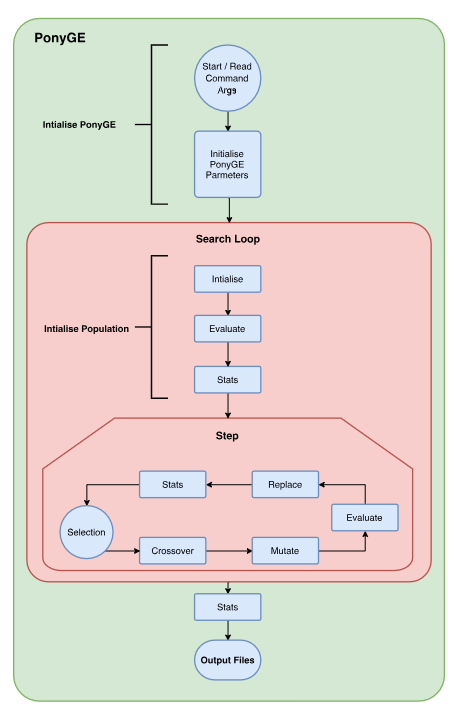
\includegraphics[scale=0.9]{figures/PonyGE2_control_flow_diagram.png}
    \caption[PonyGE2 control flow diagram.]{PonyGE2 control flow diagram \parencite{fenton2017}.}
    \label{fig:ponyge2_flow}
\end{figure}

\subsection{Genome Structure}

The genome structure is defined by codons: each codon is an integer in the range $[0, 99{,}999]$, corresponding to a codon size of 100{,}000.
Because the production is chosen with the modulo of the number of productions, which is 6 here, a large codon size makes every production equally likely for a random codon and lets mutation move freely between them.
The maximum genome length (\texttt{MAX\_GENOME\_LENGTH}) is 500 codons and represents the maximum ``DNA length'' of an individual; it prevents the genomes from growing without bound through crossover, which can produce offspring longer than their parents.
Genome wrapping is disabled (\texttt{MAX\_WRAPS} $= 0$): when a derivation needs more codons than the genome contains, the individual is invalid instead of reusing the genome from the start.
Invalid individuals receive no fitness and are not chosen as parents (\texttt{INVALID\_SELECTION} is false).

Since each codon decides one node, the length of the genome bounds the number of nodes of a hierarchy.
The largest hierarchy splits every branch on all five features, starting with the feature with most values; it has $1 + 5 + 5\cdot4 + 5\cdot4\cdot3 + 5\cdot4\cdot3\cdot2 + 240 = 446$ nodes, excluding truncated branches, and the useful hierarchies found are much smaller.
A cap of 500 codons is therefore above what such hierarchies require: it stops bloat without cutting off valid hierarchies.
The derivation depth is further limited by \texttt{MAX\_TREE\_DEPTH} $= 20$.
A useful hierarchy is at most five levels deep, since a feature repeated on a path is truncated, so this limit only constrains the truncated, non-functional branches.

\subsection{Search Operators and Parameters}

Table~\ref{tab:ge-params} lists the configuration of the experimental campaign and the role of each parameter; the operators themselves are described in Chapter~2.

\begin{table}[htbp]
    \centering
    \caption{Key Configuration Parameters (experimental campaign)}
    \label{tab:ge-params}
    \begin{tabularx}{\textwidth}{llX}
        \toprule
        Parameter & Value & Role in this work \\
        \midrule
        CODON\_SIZE & 100000 & Range of each codon, $[0, 99{,}999]$. \\
        MAX\_GENOME\_LENGTH & 500 & Upper bound on the genome; prevents bloat. \\
        MAX\_WRAPS & 0 & No wrapping: an incomplete derivation is invalid. \\
        INITIALISATION & PI\_grow & Initial trees grown in random order, at least one branch reaching the maximum initial depth. \\
        MAX\_INIT\_TREE\_DEPTH & 5 & Initial hierarchies can already use all five features. \\
        MAX\_TREE\_DEPTH & 20 & Limit on the depth of the derivation tree. \\
        POPULATION\_SIZE & 10 & Individuals per generation; small because of the cost of the fitness. \\
        GENERATIONS & 50 & Number of generations, giving 510 evaluations per run. \\
        SELECTION & tournament & Parents chosen by tournaments among random individuals. \\
        TOURNAMENT\_SIZE & 2 & Low selection pressure, which preserves diversity in a small population. \\
        CROSSOVER & variable\_onepoint & Tails of two parents swapped after independent cut points; offspring length may change. \\
        CROSSOVER\_PROBABILITY & 0.75 & Share of parent pairs that undergo crossover. \\
        MUTATION & int\_flip\_per\_codon & Each used codon replaced by a random integer with probability $1/\text{(number of used codons)}$, i.e.\ about one change per individual. \\
        REPLACEMENT & generational & The offspring replace the population in every generation. \\
        ELITE\_SIZE & 1 & The best individual is copied unchanged to the next generation. \\
        FITNESS\_FUNCTION & hierarchy\_auc & Weighted \ac{AUC} of Equation~\eqref{eq:weighted-auc-ch4} on the training period. \\
        \bottomrule
    \end{tabularx}
\end{table}

Two parameters deserve a comment.
Mutation is applied only to the used codons, that is, to the part of the genome that was read during the mapping, so every mutation changes a decision that is actually part of the hierarchy.
Because codons are read depth first, a mutation near the start of the genome changes a split close to the root and alters the meaning of all the codons that follow; a mutation near the end changes only one small branch.
The search therefore makes both large and small structural moves.
Elitism guarantees that the best fitness never decreases from one generation to the next, so the best individual of the final generation is also the best individual found in the run; this is the hierarchy reported for each run in Chapter~\ref{chap:results}.

The population size and the number of generations are much smaller than the PonyGE2 defaults and than the values in \texttt{parameters/mobai.txt} (50 and 100).
Each evaluation builds every leaf series from about 630{,}000 records and computes one \ac{MP} per valid leaf, so the budget had to be reduced to complete ten independent runs (Section~\ref{sec:tools}).
PonyGE2 caches the fitness of every phenotype already evaluated, so duplicates produced by elitism or by neutral mutations of truncated branches are not scored twice.

\section{Technological Tools and Computational Environment}
\label{sec:tools}

This section describes the technological tools used in this dissertation, the parts of the implementation that were reused and developed, and the environment in which the experimental campaign was run.
The whole pipeline, from data aggregation to the statistical tests, was implemented in Python.
This choice follows from the two core components of the method: PonyGE2 \parencite{fenton2017} and STUMPY \parencite{law2019stumpy} are both Python libraries, so the search, the scorer and the evaluation share one language and one data representation.
Table~\ref{tab:tools} lists the tools and the versions used in the experimental campaign.

\begin{table}[H]
    \centering
    \caption{Technological tools employed}
    \label{tab:tools}
    \begin{tabularx}{\textwidth}{llX}
        \toprule
        Name & Version & Role in this work \\
        \midrule
        Python & 3.13.11 & Programming language of the whole pipeline. \\
        PonyGE2 & fork & \ac{GE} engine: genotype-to-phenotype mapping through the grammar, initialisation, selection, crossover, mutation, replacement and logging of each run. \\
        STUMPY & 1.14.1 & Computation of the \ac{MP} of each leaf series with \texttt{stumpy.stump}. \\
        Numba & 0.66.0 & Just-in-time compiler used by STUMPY to run the \ac{MP} kernels as native code. \\
        pandas & 2.3.3 & Loading of the CSV datasets, filtering of the records of each leaf, hourly aggregation and alignment to the full hourly index. \\
        NumPy & 2.4.4 & Array operations, including the first difference and min--max normalisation of the \ac{MP}. \\
        scikit-learn & 1.8.0 & \ac{ROC} \ac{AUC} (\texttt{roc\_auc\_score}) and precision, recall and F1 of the pooled evaluation. \\
        SciPy & 1.17.1 & Wilcoxon signed-rank tests against the baselines. \\
        Matplotlib & 3.11.2 & Figures of Chapter~\ref{chap:results}. \\
        Kaggle Notebooks & -- & Hosted Jupyter environment used for data preparation, exploratory analysis, enumeration of the feature combinations, anomaly injection and early prototypes of the hierarchy and \ac{MP} scoring. \\
        \bottomrule
    \end{tabularx}
\end{table}

\subsection{Reused and Developed Components}

PonyGE2 is used as the search engine with its standard operators; the only changes to the framework replace the deprecated constant \texttt{np.NaN} with \texttt{np.nan} in \texttt{mapper.py} and \texttt{base\_ff.py}, which is required by NumPy~2 and does not change its behaviour.
The components specific to this problem were developed for this dissertation:
\begin{itemize}
    \item the grammar \texttt{grammars/mobai\_nop.pybnf}, which defines the space of admissible hierarchies (Section~\ref{sec:grammar});
    \item the fitness function \texttt{src/fitness/hierarchy\_auc.py}, which loads the training set once and evaluates each individual (Section~\ref{sec:fitness-evaluation});
    \item \sloppy the module \path{src/fitness/mobai_utils.py}, which parses the phenotype (\texttt{pheno\_to\_dict}), builds and aligns the leaf series (\texttt{create\_final\_hierarchy}, \texttt{set\_leaf}), scores them (\texttt{leaf\_scores}) and computes the weighted \ac{AUC} (\texttt{calculate\_AUC\_hierarchy});
    \item the script \texttt{src/evaluate\_experiment.py}, which re-evaluates the best individual of every run and the seven baselines on both periods, computes the original and pooled metrics and runs the Wilcoxon tests;
    \item the script \texttt{src/plot\_results.py}, which produces the figures and tables of Chapter~\ref{chap:results} from the saved runs.
\end{itemize}
The same functions are used during the search and in the final evaluation, so the reported test values are computed exactly as the fitness, only on the test period.

The data preparation that precedes the search was carried out in Kaggle notebooks over the private operator data.
They load the raw extract, parse the timestamps, clean the \#Events column, drop the unused columns and the duplicated records, and produce the exploratory analysis of Section~\ref{sec:problem-formulation}.
They also enumerate the 94{,}080 possible combinations of the six features and separate the 1{,}555 that occur in the data, with the number of hours in which each is observed; this list is what the injection procedure checks before accepting a segment.
Finally, they implement the anomaly injection of Section~\ref{sec:anomaly-injection} and the plots used to inspect the injected anomalies.
The same notebooks also contain the early prototypes of the approach, in which hierarchies were sampled at random and scored first with a z-score heuristic and then with the \ac{MP}; these prototypes motivated the replacement of random sampling by a grammar-guided search and are not part of the reported experiments.

\subsection{Computational Environment}

The experimental campaign was run on a desktop computer with an AMD Ryzen~7 8700F processor (8 cores, 16 threads) and 32~GB of RAM, under Windows~11.
Ten independent runs were executed, one per random seed from 0 to 9, with four runs in parallel.
Within each run, PonyGE2 evaluates the individuals of a generation on four processes (\texttt{MULTICORE}, \texttt{CORES} $= 4$) and caches the fitness of phenotypes already evaluated (\texttt{CACHE}), so duplicated individuals are not scored again.
Each run took between 13 and 20 minutes.
Most of this time is spent in the fitness function, since every evaluation filters the records and computes one \ac{MP} per leaf; this cost is the reason for the reduced population size and number of generations (Section~\ref{sec:setup}).

\subsection{Reproducibility}

Every run is identified by its random seed, and PonyGE2 stores in its result folder the full parameter file used (\texttt{parameters.txt}), the statistics of every generation (\texttt{stats.tsv}) and the best individual with its phenotype (\texttt{best.txt}).
The campaign settings (population 10, 50 generations) override the defaults of \texttt{parameters/mobai.txt}, so the stored \texttt{parameters.txt} of each run is the reference for its configuration.
\begin{sloppypar}
The final evaluation reads only these folders and the fixed training and test sets (\path{datasets/Mobai/train_set.csv} and \path{test_set.csv}), and writes the results to \texttt{evaluation.csv}, \texttt{evaluation\_pooled.csv} and \texttt{results\_tables.md}, so all values reported in Chapter~\ref{chap:results} can be regenerated without repeating the search.
\end{sloppypar}

\chapter{Results and Discussion}
\label{chap:results}

This chapter reports the experimental evaluation of the aggregation hierarchies evolved with \ac{GE}.
Section~\ref{sec:setup} summarises the experimental configuration.
Section~\ref{sec:performance} compares the evolved hierarchies with seven fixed aggregation baselines under two scoring schemes.
Section~\ref{sec:ts-visualisation} illustrates the behaviour of the detector on individual series, Section~\ref{sec:ge-analysis} analyses the search process and the evolved structures, and Section~\ref{sec:discussion} discusses the findings.
Section~\ref{sec:limitations} closes the chapter with the threats to validity.

\section{Experimental Setup}
\label{sec:setup}

\subsection{Data, Split and Labels}

The experiments use the hourly \#Events series of the switch data described in Chapter~3, after synthetic anomaly injection (Figure~\ref{fig:workflow}).
The data is split temporally, without shuffling:
\begin{itemize}
    \item \textbf{Training period:} 18 July 2022 00:00 to 14 September 2022 18:00 (1{,}411 hours);
    \item \textbf{Test period:} 14 September 2022 19:00 to 13 October 2022 21:00 (699 hours).
\end{itemize}
For every leaf of a hierarchy, the filtered records are aggregated to an hourly series and aligned to the full hourly range of the split, with missing hours filled with zero.
Sparse feature combinations therefore become series that are zero for most hours.

Each injected anomaly modifies a single hour: the 168-hour window is only used to estimate the local mean $\mu$ and standard deviation $\sigma$, and the modified value is placed outside $\mu \pm 3\sigma$.
The labels are therefore \emph{point} anomalies.
Because each anomaly affects one feature combination, the share of anomalous hours depends on the granularity of the view.
In the test period it is 4.3\% for the fully aggregated series, between 1.6\% and 2.7\% for the single-category views, 0.8\% on average for the evolved hierarchies and 0.12\% for full disaggregation.

\subsection{Anomaly Scoring and Evaluation Metrics}

Each leaf series is scored with the \ac{MP} computed by STUMPY \parencite{law2019stumpy} with a window of $m = 168$ hours (one week).
The anomaly score of each hour is the first difference of the matrix profile, min--max normalised to $[0, 1]$.
Since no complete window exists for the first $m$ hours of a split, these hours are not scored and their labels are ignored.

Two metrics are reported.
The first, used as fitness during the search, is the event-weighted mean of the leaf \ac{AUC}s:
\begin{equation}
    \mathrm{AUC}_{H} = \sum_{\ell \in \mathcal{V}} w_\ell \, \mathrm{AUC}_\ell,
    \qquad
    w_\ell = \frac{E_\ell}{\sum_{k \in \mathcal{V}} E_k},
    \label{eq:weighted-auc}
\end{equation}
where $\mathrm{AUC}_\ell$ is the \ac{ROC} \ac{AUC} of leaf $\ell$, $E_\ell$ its total number of events, and $\mathcal{V}$ the set of leaves that contain both normal and anomalous hours after the first $m$ hours.
Leaves without anomalies are excluded from $\mathcal{V}$, so false alarms raised on them do not affect the metric.
This is referred to as the \emph{original} metric.

As a robustness check, a \emph{pooled} \ac{AUC} is also computed: the scores and labels of all leaves are concatenated into a single \ac{ROC} curve, so anomaly-free leaves contribute negatives and their false alarms are counted.
On the same pooled scores, the hours in the top 5\% of scores are flagged as anomalous, and precision, recall and F1 are reported.
The 5\% threshold matches the injection rate and is deliberately generous given the label rates above.

\subsection{Search Configuration}

The search uses PonyGE2 \parencite{fenton2017} with the grammar \texttt{mobai\_nop.pybnf}, which covers five categorical features (Call, Event, Subscriber, Traffic and Service Type).
Partner Description is excluded because of its high entropy (8.4 bits, Chapter~\ref{chap:methodology}).
Table~\ref{tab:ge-config} lists the configuration used in the experimental campaign.
Population size and number of generations were reduced to 10 and 50 because of the computational budget: each fitness evaluation builds and scores every leaf of a hierarchy.
Each run took between 13 and 20 minutes with four runs in parallel.

\begin{table}[htbp]
    \centering
    \caption{Configuration of the experimental campaign}
    \label{tab:ge-config}
    \begin{tabular}{ll}
        \toprule
        Parameter & Value \\
        \midrule
        Grammar & \texttt{mobai\_nop.pybnf} (5 features) \\
        Population size & 10 \\
        Generations & 50 (510 evaluations per run) \\
        Independent runs & 10 (random seeds 0--9) \\
        Initialisation & \ac{PIG}, maximum initial depth 5 \\
        Maximum tree depth & 20 \\
        Maximum genome length & 500 codons \\
        Codon size & 100{,}000 \\
        Selection & Tournament, size 2 \\
        Crossover & Variable one-point, probability 0.75 \\
        Mutation & Integer flip per codon \\
        Replacement & Generational, with elitism \\
        Fitness & $\mathrm{AUC}_H$ (Equation~\ref{eq:weighted-auc}) on the training period \\
        \bottomrule
    \end{tabular}
\end{table}

For each run, the best individual of the final generation is evaluated on both periods.
When a single evolved hierarchy is analysed in detail, the run with the highest \emph{training} fitness is used (seed 7); selecting by test performance would leak information from the test set.

\subsection{Baselines and Statistical Testing}

The evolved hierarchies are compared with seven fixed hierarchies:
\begin{itemize}
    \item \textbf{Fully aggregated:} a single series with all traffic;
    \item \textbf{By Call Type} (2 leaves), \textbf{By Event Type} (4), \textbf{By Subscriber Type} (5), \textbf{By Traffic Type} (3) and \textbf{By Service Type} (2): one split on a single feature;
    \item \textbf{Fully disaggregated:} the 1{,}555 non-empty feature combinations, including Partner Description.
\end{itemize}
The single-feature baselines can also be generated by the grammar, so the search could, in principle, reach them.

The baselines are deterministic and are evaluated once.
The ten evolved hierarchies are compared with each baseline using a two-sided one-sample Wilcoxon signed-rank test on the differences in test \ac{AUC}.
With ten runs, the smallest attainable $p$-value is 0.002, which occurs when all ten runs lie on the same side of the baseline.

\section{Performance Analysis}
\label{sec:performance}

\subsection{Comparison with Fixed Baselines}

Table~\ref{tab:auc-main} and Figures~\ref{fig:auc-baselines-train} and~\ref{fig:auc-baselines-test} report the original metric on the training and test periods.
The evolved hierarchies reach a test \ac{AUC} of $0.678 \pm 0.066$ (median 0.655, range 0.598--0.778).
They are significantly better than four baselines: the fully aggregated series and the Call, Event and Service Type splits, by 0.10 to 0.14 \ac{AUC} ($p = 0.002$).
They are statistically indistinguishable from the Traffic Type split ($p = 0.92$), and worse than the Subscriber Type split ($-0.056$, $p = 0.027$) and full disaggregation ($-0.198$, $p = 0.002$).

\begin{table}[htbp]
    \centering
    \caption[ROC-AUC of evolved hierarchies and fixed baselines (original metric)]{\ac{ROC}-\ac{AUC} of the best evolved hierarchy per run and of the fixed baselines, using the event-weighted metric over leaves containing anomalies. For the evolved hierarchies, values are mean $\pm$ standard deviation over 10 runs; $\Delta$ is the mean difference in test \ac{AUC} (evolved minus baseline). The best value of each metric is in bold.}
    \label{tab:auc-main}
    \begin{tabular}{lrcccc}
        \toprule
        Hierarchy & Leaves & Train AUC & Test AUC & $\Delta$ & Wilcoxon $p$ \\
        \midrule
        GE (10 runs) & 8--34 & $0.765 \pm 0.019$ & $0.678 \pm 0.066$ & -- & -- \\
        Fully aggregated & 1 & 0.601 & 0.543 & $+0.135$ & 0.002 \\
        By Call Type & 2 & 0.683 & 0.562 & $+0.116$ & 0.002 \\
        By Event Type & 4 & 0.669 & 0.580 & $+0.098$ & 0.002 \\
        By Service Type & 2 & 0.642 & 0.574 & $+0.104$ & 0.002 \\
        By Traffic Type & 3 & 0.614 & 0.684 & $-0.006$ & 0.92 \\
        By Subscriber Type & 5 & 0.628 & 0.734 & $-0.056$ & 0.027 \\
        Fully disaggregated & 1{,}555 & \textbf{0.791} & \textbf{0.877} & $-0.198$ & 0.002 \\
        \bottomrule
    \end{tabular}
\end{table}

\begin{figure}[htbp]
    \centering
    \includefig[width=0.85\textwidth]{figures/results/auc_vs_baselines_train.png}
    \caption[Training AUC of evolved hierarchies and fixed baselines]{Training \ac{AUC} (18 July--14 September 2022) of the fixed baselines (grey circles) and distribution of the training \ac{AUC} of the best evolved hierarchy over 10 runs (box plot and red points).}
    \label{fig:auc-baselines-train}
\end{figure}

\begin{figure}[htbp]
    \centering
    \includefig[width=0.85\textwidth]{figures/results/auc_vs_baselines_test.png}
    \caption[Test AUC of evolved hierarchies and fixed baselines]{Test \ac{AUC} (14 September--13 October 2022) of the fixed baselines (blue diamonds) and distribution of the test \ac{AUC} of the best evolved hierarchy over 10 runs (box plot and red points). Rows and horizontal axis are the same as in Figure~\ref{fig:auc-baselines-train}.}
    \label{fig:auc-baselines-test}
\end{figure}

Two baselines, Subscriber Type and Traffic Type, score higher on the test period than on the training period.
The two periods therefore differ in how detectable the injected anomalies are, which is relevant to the generalisation analysis below.

\subsection{Robustness Check: Pooled Scoring}

Table~\ref{tab:pooled} and Figure~\ref{fig:pooled-original} report the pooled metric, in which false alarms on anomaly-free leaves are counted.
The ranking of the hierarchies changes substantially.
Full disaggregation drops from 0.877 to 0.600, and its precision among the top 5\% of scores is only 0.4\%: roughly 250 false alarms are raised for each correctly flagged anomalous hour.
The Subscriber Type split drops from 0.734 to 0.581, while the Event Type and Service Type splits rise to about 0.72.

\begin{table}[htbp]
    \centering
    \caption[Pooled ROC-AUC and threshold metrics on the test period]{Pooled \ac{ROC}-\ac{AUC} over all leaf-hours and precision, recall and F1 when the top 5\% of scores are flagged (test period). For the evolved hierarchies, values are means over 10 runs; $p$ is the Wilcoxon signed-rank $p$-value of the difference $\Delta$. The best value of each metric is in bold.}
    \label{tab:pooled}
    \begin{tabular}{lcccccc}
        \toprule
        Hierarchy & Pooled AUC & $\Delta$ & $p$ & Precision & Recall & F1 \\
        \midrule
        GE (10 runs) & $0.670 \pm 0.039$ & -- & -- & 0.050 & 0.308 & 0.086 \\
        Fully aggregated & 0.543 & $+0.127$ & 0.002 & 0.107 & 0.130 & 0.118 \\
        By Call Type & 0.510 & $+0.160$ & 0.002 & 0.056 & 0.103 & 0.072 \\
        By Event Type & 0.715 & $-0.046$ & 0.010 & 0.083 & 0.220 & 0.121 \\
        By Service Type & \textbf{0.717} & $-0.048$ & 0.010 & 0.074 & 0.154 & 0.100 \\
        By Traffic Type & 0.690 & $-0.021$ & 0.16 & \textbf{0.125} & \textbf{0.323} & \textbf{0.180} \\
        By Subscriber Type & 0.581 & $+0.088$ & 0.002 & 0.060 & 0.186 & 0.091 \\
        Fully disaggregated & 0.600 & $+0.069$ & 0.002 & 0.004 & 0.165 & 0.008 \\
        \bottomrule
    \end{tabular}
\end{table}

\begin{figure}[htbp]
    \centering
    \includefig[width=\textwidth]{figures/results/pooled_vs_original.png}
    \caption[Original vs pooled test AUC]{Test \ac{AUC} under the original metric (leaves with anomalies only) and the pooled metric (all leaves). Error bars show the standard deviation over the 10 evolved hierarchies.}
    \label{fig:pooled-original}
\end{figure}

The mean pooled \ac{AUC} of the evolved hierarchies ($0.670$) is close to their original test \ac{AUC} ($0.678$).
Under pooled scoring they remain significantly better than the fully aggregated series, the Call and Subscriber Type splits and full disaggregation, are indistinguishable from the Traffic Type split ($p = 0.16$), and are slightly worse than the Event and Service Type splits ($-0.05$, $p = 0.010$).
The ordering of the runs, however, changes: seeds 6 and 7, the best two runs under the original metric, have the lowest pooled \ac{AUC} (0.606 and 0.623), while seeds 0, 1 and 9 perform best (0.70 to 0.72).

F1 is low for every hierarchy (at most 0.18).
This follows from the label rates of 0.1\% to 4.3\% of hours and the 5\% threshold, which bounds precision from above, and F1 is therefore not used as the main comparison.

\subsection{Hierarchy Size and Detection Quality}

Figure~\ref{fig:leaves-auc} relates the number of leaf series to the test \ac{AUC}.
The evolved hierarchies contain between 8 and 34 leaves (19.6 on average).
Under the original metric, the only hierarchy that clearly outperforms them requires 1{,}555 series.
Under pooled scoring, however, two single-feature splits with two to four leaves perform as well or slightly better.

\begin{figure}[htbp]
    \centering
    \includefig[width=0.75\textwidth]{figures/results/leaves_vs_auc.png}
    \caption[Test AUC against number of leaf series]{Test \ac{AUC} (original metric) against the number of leaf series to monitor, on a logarithmic scale.}
    \label{fig:leaves-auc}
\end{figure}

\subsection{Generalisation}

Figure~\ref{fig:train-test} compares training and test \ac{AUC}.
Seven of the ten runs lose between 0.10 and 0.15 \ac{AUC} on the test period, while seeds 6, 7 and 9 hold up (0.76 to 0.78).
Training fitness is a weak guide to test performance: across runs, the Spearman correlation between training \ac{AUC} and pooled test \ac{AUC} is $-0.27$, and between original and pooled test \ac{AUC} it is $0.20$; neither is significant.

\begin{figure}[htbp]
    \centering
    \includefig[width=0.6\textwidth]{figures/results/train_vs_test.png}
    \caption[Train vs test AUC]{Training against test \ac{AUC} (original metric) for each evolved hierarchy and baseline. Points below the diagonal lose \ac{AUC} on the test period.}
    \label{fig:train-test}
\end{figure}

\section{Time Series Visualisation}
\label{sec:ts-visualisation}

Figure~\ref{fig:ts-examples} shows the test period for three leaves of the best evolved hierarchy (seed 7) and for the fully aggregated series.
The three leaves were selected by rank, as the leaves with the best, median and worst leaf \ac{AUC}, rather than chosen for visual appeal.

\begin{figure}[htbp]
    \centering
    \includefig[width=\textwidth]{figures/results/ts_leaf_examples.png}
    \caption[Leaf series, labelled anomalies and Matrix Profile scores]{Test period for the best, median and worst leaf of the best evolved hierarchy (seed 7) and for the fully aggregated series. Blue: hourly \#Events; orange: labelled anomalous hours; red: normalised \ac{MP} score ($m = 168$).}
    \label{fig:ts-examples}
\end{figure}

\begin{itemize}
    \item \textbf{Best leaf} (TERMINATED / ON-NET / VOICE / Prepaid, \ac{AUC} 1.00): a high-volume, regular series. The injected value is a clear discord and the score peaks at the labelled hour.
    \item \textbf{Median leaf} (TERMINATED / INT / Other, \ac{AUC} 0.73): a noisier series in which some anomalies are detected and others are missed.
    \item \textbf{Worst leaf} (ORIGINATED / VOICE / Roamer In / OFF-NET, \ac{AUC} 0.03): a sparse series with 0 to 4 events per hour. The injected value is indistinguishable from the normal spikes, so the \ac{MP} cannot separate it.
    \item \textbf{Fully aggregated series} (\ac{AUC} 0.54): many hours are labelled, but each anomaly originates in a small subgroup and is hidden in the total. This illustrates the dilution effect that motivates searching for an intermediate level of aggregation.
\end{itemize}

Two properties of the scorer are also visible.
Anomalies in the first week are never scored, because the score starts at hour 168.
Because the score is a first difference of the matrix profile, it produces a positive spike where a discord begins and a drop where it ends.

\section{Genetic Programming Analysis}
\label{sec:ge-analysis}

\subsection{Fitness Evolution}

Figure~\ref{fig:fitness} shows the best and average training fitness per generation.
The mean best fitness rises from 0.710 in the initial population to 0.765 after 50 generations, and the population average from 0.658 to about 0.73.
Most of the improvement happens in the first eight generations and is followed by long plateaus, as expected for a population of ten individuals with tournament size 2.
The search had not converged: several runs still improve after generation 40, for example seed 7 at about generation 43.
More generations would likely increase training fitness, but, given the generalisation gap reported above, not necessarily test performance.

\begin{figure}[htbp]
    \centering
    \includefig[width=0.75\textwidth]{figures/results/fitness_evolution.png}
    \caption[Fitness evolution]{Best training fitness per generation for each of the 10 runs (faint lines), their mean (solid) and the mean population average (dashed).}
    \label{fig:fitness}
\end{figure}

\subsection{Best Evolved Hierarchy}

Figure~\ref{fig:phenotype-tree} shows the hierarchy evolved by seed 7, which has the highest training fitness (0.802; test 0.772).
It contains 34 leaves, splits first on Event Type, and uses up to five conditions per leaf.

\begin{figure}[htbp]
    \centering
    \includefig[width=0.88\textwidth]{figures/results/phenotype_tree.png}
    \caption[Best evolved hierarchy (seed 7)]{Hierarchy evolved by seed 7. Each path from the root to a leaf is a conjunction of filters, with boxes coloured by feature. Leaves are coloured by test \ac{AUC} and sized by their weight $w_\ell$ in Equation~\ref{eq:weighted-auc}; leaves without both classes in the test period are not scored.}
    \label{fig:phenotype-tree}
\end{figure}

\begin{itemize}
    \item The tree is asymmetric: it splits deeply where traffic is heterogeneous (ORIGINATED / VOICE and TERMINATED / INT) and stops early where it is not (ROAMING OUT has a single further split).
    \item The CALL FORWARD branch yields near-perfect leaves (\ac{AUC} 0.95 to 1.00), but these carry little weight because the volume is concentrated elsewhere.
    \item The three worst leaves all belong to Roamer In traffic (\ac{AUC} 0.03, 0.12 and 0.41); these are sparse, bursty series of the kind discussed in Section~\ref{sec:ts-visualisation}.
    \item A single leaf, TERMINATED / ON-NET / SMS, carries 43\% of the weight with an \ac{AUC} of 0.73, so the score of the hierarchy is largely the score of this series.
    \item Nine of the 34 leaves are not scored in the test period. Seven contain no anomaly at all and two contain an anomaly only in the unscored first week. Their false alarms do not affect the original metric.
\end{itemize}

\subsection{Structure Across Runs}

Table~\ref{tab:structure} summarises the best hierarchy of each run.

\begin{table}[htbp]
    \centering
    \caption[Structure of the best evolved hierarchy per run]{Structure of the best evolved hierarchy per run. Depth is the maximum number of conditions in a leaf; unused features are those of the five grammar features that never appear in a filter. Train, test and pooled test values are \ac{AUC}s.}
    \label{tab:structure}
    \begin{tabular}{crcllccc}
        \toprule
        Seed & Leaves & Depth & Root split & Unused features & Train & Test & Pooled \\
        \midrule
        0 & 15 & 3 & Call Type & Service & 0.760 & 0.658 & 0.720 \\
        1 & 22 & 4 & Call Type & -- & 0.772 & 0.649 & 0.704 \\
        2 & 17 & 4 & Call Type & Traffic & 0.766 & 0.631 & 0.659 \\
        3 & 19 & 5 & Call Type & -- & 0.772 & 0.657 & 0.681 \\
        4 & 21 & 4 & Call Type & -- & 0.768 & 0.654 & 0.678 \\
        5 & 8 & 3 & Call Type & Event, Traffic & 0.728 & 0.627 & 0.653 \\
        6 & 22 & 4 & Event Type & -- & 0.773 & 0.758 & 0.606 \\
        7 & 34 & 5 & Event Type & -- & 0.802 & 0.772 & 0.623 \\
        8 & 14 & 4 & Service Type & Traffic & 0.745 & 0.598 & 0.649 \\
        9 & 24 & 5 & Call Type & -- & 0.761 & 0.778 & 0.724 \\
        \bottomrule
    \end{tabular}
\end{table}

\begin{itemize}
    \item Call Type is the root split in seven of the ten runs. With two values (SMS and VOICE), it is the cheapest first split.
    \item Every run uses Call Type and Subscriber Type. Traffic Type is absent from the three runs with the lowest test \ac{AUC} (seeds 2, 5 and 8), which, together with the strong Traffic Type baseline, suggests that this feature carries useful structure.
    \item Leaves use three to five conditions. Five is the maximum by construction: there are five features, and a branch is truncated when a feature repeats along a path. Derivation trees of up to 20 levels therefore collapse to at most five effective levels.
    \item There is no common best structure. The hierarchies differ widely between runs, yet several reach similar fitness, which indicates a flat fitness landscape with many near-equivalent structures. This favours interpretability, since a readable structure can be chosen among equivalent ones, but limits the stability of the result.
\end{itemize}

\section{Discussion}
\label{sec:discussion}

\subsection{Research Objectives}

The objectives in Chapter~1 can be answered as follows.

\begin{itemize}
    \item \textbf{Can aggregation choice be framed as a combinatorial search over a grammar?}
    Yes. Every individual that maps successfully is a valid hierarchy, and PonyGE2 found hierarchies with 8 to 34 leaves within 510 evaluations per run.
    \item \textbf{Can a label-free \ac{MP} scorer drive the search?}
    Partly. With the detector fixed, the choice of aggregation alone moves the test \ac{AUC} between 0.54 and 0.88 under the original metric, so the scorer clearly discriminates between views. However, the event-weighted fitness can be exploited, as discussed in Section~\ref{sec:metric-sensitivity}.
    \item \textbf{Do evolved hierarchies outperform fixed aggregation?}
    They robustly outperform the coarse fixed views (the fully aggregated series and the Call Type split) under both metrics. They do not outperform the best single-feature splits, and whether they outperform full disaggregation depends on the metric.
\end{itemize}

\subsection{Sensitivity to the Evaluation Metric}
\label{sec:metric-sensitivity}

The same hierarchies rank differently under the two metrics, which is the main methodological finding of this work.
Under the original metric, full disaggregation is the best hierarchy (0.877); under pooled scoring it falls below the evolved hierarchies (0.600).
The reason is the exclusion of anomaly-free leaves from Equation~\ref{eq:weighted-auc}: with 1{,}555 leaves, most leaves contain no anomaly, and the false alarms raised on them are not counted.
The precision of 0.4\% among the top 5\% of scores shows the operational cost hidden by the original metric.

The same mechanism affects the search.
Seeds 6 and 7, which score highest under the original metric, score lowest under pooled scoring, which suggests that the fitness rewards hierarchies that concentrate anomalies in a few leaves and leave many normal-only leaves that drop out of the score.
A fitness that counts false alarms in every leaf, such as the pooled \ac{AUC}, avoids this and is cheap to compute.

\subsection{Generalisation Gap}

The training and test periods behave differently: the Subscriber Type split scores 0.628 on the training period and 0.734 on the test period.
Because the search optimises the training period only, without a validation split, it selects structures that fit the anomalies injected in that period.
A validation window or rolling-origin evaluation of the fitness, larger populations, or averaging the fitness over several injection seeds could reduce this gap.

\subsection{Parsimony and Interpretability}

The evolved hierarchies require about 20 monitored series, compared with 1{,}555 for full disaggregation, and under pooled scoring they are also more accurate.
Each leaf is a readable conjunction of business filters, such as TERMINATED / ON-NET / SMS, so an alert can be traced directly to a traffic segment.
The contribution of the search is therefore competitive detection with a small, interpretable set of series, found without knowing in advance which feature to split on, rather than the best detection overall.

\subsection{Behaviour of the Matrix Profile Scorer}

The \ac{MP} scorer works well on large, regular series with strong weekly seasonality, reaching leaf \ac{AUC}s of 1.00.
It fails on sparse integer series, such as the Roamer In leaves.
A likely cause is that z-normalised subsequences consisting mostly of zeros make every isolated spike look like a discord, so injected and normal spikes cannot be distinguished.
This supports excluding very sparse feature combinations, for example with a minimum-support rule in the grammar.

\subsection{Relation to Previous Work}

Telecom anomaly detection studies typically evaluate detectors on a fixed view of the data \parencite{gonzalez2024one, mefleh2025beyond, burgueno2020online}.
The results above show that, with the detector held fixed, the view alone changes the test \ac{AUC} by up to 0.33, which supports treating aggregation as a search problem.
Hierarchical search \parencite{wolff2022composite} and subspace mining \parencite{he2021mining} also search over structure, but neither uses a grammar or \ac{MP}-based scoring.
The \ac{MP} literature presents the matrix profile as a strong, parameter-light discord detector \parencite{yeh2017timeseriesjoins}; the present results agree for dense series and add a failure case for sparse ones.
The \ac{AUC} values reported here are computed on synthetic point anomalies and are not directly comparable with F1 or range-based F1 scores obtained on expert labels in those studies.

\section{Limitations}
\label{sec:limitations}

\begin{itemize}
    \item Only synthetic point anomalies are evaluated; real incidents may be longer, collective or contextual.
    \item A single dataset and a single temporal split are used, without cross-validation over time.
    \item The search budget is small (population 10, 50 generations, 10 runs) and the search had not converged.
    \item Partner Description is excluded from the grammar but included in the fully disaggregated baseline, so that comparison is not like-for-like.
    \item The original fitness ignores false alarms in anomaly-free leaves, and event-volume weighting allows a single leaf to dominate (43\% of the weight for seed 7).
    \item The 5\% threshold for the threshold metrics is arbitrary relative to label rates of 0.1\% to 4.3\%.
    \item Labels in the first 168 hours of each split are never scored.
    \item Only one score definition, the first difference of the matrix profile, was tested; the raw matrix profile and its absolute difference were not compared.
\end{itemize}

\chapter{Conclusions and Future Works}
\label{chap:conclusions}

\section{Conclusions}

This dissertation addressed a practical question in the monitoring of mobile networks: at which level of aggregation should telecommunications traffic be analysed to detect anomalies?
A fully aggregated series hides anomalies that affect a small segment of the traffic, while one series per combination of categories produces too many sparse series to monitor and interpret.
Instead of fixing the aggregation in advance, this work treated it as a combinatorial search.
Candidate hierarchies were generated by a \ac{BNF} grammar over the categorical features of the traffic, evolved with \ac{GE} in PonyGE2, and ranked by how well a label-free Matrix Profile detector found synthetic anomalies in the series they produced.

The framework was applied to hourly \#Events from a mobile network switch, covering July to October 2022, with about one million records and six categorical features.
Because the operational data has no reliable anomaly labels, 105 point anomalies were injected at three standard deviations from the local weekly mean, each in a randomly chosen segment of the traffic.
The data analysis showed that the traffic is highly concentrated: a few combinations carry most of the events, while most of the 1{,}555 non-empty combinations are small and sparse.
Partner Description, with 392 values and the highest entropy, was therefore excluded from the grammar, which kept the search space manageable and avoided splits that produce hundreds of nearly empty series.

The main conclusions are the following.

\begin{itemize}
    \item \textbf{Aggregation matters as much as the detector.}
    With the detector held fixed, the choice of aggregation alone changed the test \ac{AUC} from 0.54 for the fully aggregated series to 0.88 for full disaggregation.
    The injection experiments also showed why: an anomaly that is obvious in its own segment is diluted, and often invisible, in any series that also contains other traffic.
    This supports the premise of the dissertation that the view of the data should be chosen, and not assumed.

    \item \textbf{A grammar is a practical way to define the search space.}
    The grammar generates only valid hierarchies, each leaf is a readable conjunction of business filters, and the leaves always partition the traffic, so no repair or penalty is needed.
    The space it defines contains about $2.2 \times 10^{61}$ distinct hierarchies, which rules out exhaustive search, yet PonyGE2 found hierarchies with 8 to 34 leaves in 510 evaluations per run.

    \item \textbf{The evolved hierarchies are competitive, but not the best overall.}
    They reached a test \ac{AUC} of $0.678 \pm 0.066$ and were significantly better than the fully aggregated series and the Call, Event and Service Type splits.
    They did not outperform the best single-feature splits, and under the original metric full disaggregation was better.
    Their advantage is a compact, interpretable set of about 20 series that is found without knowing in advance which features to split on.

    \item \textbf{The evaluation metric changes the conclusions.}
    The event-weighted \ac{AUC} used as fitness ignores leaves without anomalies, so false alarms on those leaves are not counted.
    When they are counted, with a pooled \ac{AUC}, full disaggregation falls from 0.877 to 0.600, with a precision of 0.4\%, while the evolved hierarchies keep a similar value (0.670).
    The two runs with the best original fitness had the lowest pooled \ac{AUC}, which shows that the search can exploit this blind spot of the fitness function.
    This is the main methodological finding of the work.

    \item \textbf{The Matrix Profile works well on dense series and fails on sparse ones.}
    On high-volume series with a regular weekly shape, the first difference of the profile located the injected anomalies with leaf \ac{AUC}s up to 1.00.
    On sparse series with a few events per hour, such as inbound roaming segments, every isolated spike looks like a discord and the detector performed worse than random.
    Which leaves a hierarchy creates therefore determines not only how visible the anomalies are but also whether the detector can work at all.

    \item \textbf{Training fitness was a weak guide to test performance.}
    Most runs lost 0.10 to 0.15 \ac{AUC} on the test period, and the fitness landscape was flat, with very different hierarchies reaching similar fitness.
    The small search budget, ten individuals for 50 generations, also meant that the search had not converged.
\end{itemize}

The contributions of this dissertation are, first, the formulation of aggregation choice for anomaly detection in grouped telecommunications series as a grammar-based search, with a fitness built from a label-free detector and synthetic anomalies; second, an implementation in Python on top of PonyGE2 and STUMPY that evaluates candidate hierarchies on real operator data and can be reproduced from the saved runs; and third, an empirical analysis that compares evolved and fixed hierarchies under two metrics and shows that conclusions about the best aggregation depend strongly on how false alarms are counted.
For a network operations team, the practical message is that monitoring at an intermediate level of aggregation, chosen with the data, gives a small number of interpretable series in which anomalies are more visible than in the total, as long as sparse segments are avoided.

\section{Future Work}

The results and limitations of this work suggest several directions.

\begin{itemize}
    \item \textbf{A fitness that counts false alarms.}
    The most direct improvement is to use the pooled \ac{AUC}, or another metric that includes anomaly-free leaves, as the fitness.
    It is cheap to compute and would remove the incentive, observed in the best runs, to create many normal-only leaves.
    Precision-oriented metrics, such as the precision–recall \ac{AUC} or F1 at an operational alarm budget, are also worth testing.

    \item \textbf{Control of sparse leaves.}
    Since the Matrix Profile fails on sparse series, a minimum-support rule could stop a branch when its traffic falls below a threshold, either in the grammar or in the fitness function.
    A multi-objective formulation could additionally trade detection quality against the number of leaves, making the cost of monitoring an explicit objective.

    \item \textbf{A larger search budget and a study of stability.}
    With more individuals and generations, it would be possible to establish whether the search converges, how sensitive it is to the random seed, and whether the flat fitness landscape contains a stable core of useful splits.

    \item \textbf{Real incidents and other anomaly types.}
    Only synthetic point anomalies were evaluated.
    Validating the evolved hierarchies against real incident records from the operator, and injecting collective or contextual anomalies that last several hours, would show whether the conclusions hold for the anomalies that matter in operation.

    \item \textbf{More robust validation over time.}
    A single temporal split was used.
    Rolling-origin evaluation over several periods, and data from months beyond July to October 2022, would give a better estimate of how well an evolved hierarchy generalises and how often it needs to be re-evolved.

    \item \textbf{Reintroducing Partner Description.}
    The partner feature was excluded because of its cardinality.
    Grouping partners, for example keeping the most frequent ones and merging the long tail into a single category, would let the search use this information without creating hundreds of sparse branches.

    \item \textbf{Other scores and detectors.}
    Only the first difference of the Matrix Profile was tested.
    The raw profile and alternative detectors, such as forecast residuals or autoencoders, could be plugged into the same fitness function, keeping \ac{GE} for the structure search and testing whether the best aggregation depends on the detector.

    \item \textbf{Additional targets.}
    Only \#Events was used.
    Event Duration could be added as a second target, either as a separate search or as a second objective, since some faults may affect call length without changing the number of calls.

    \item \textbf{Towards operation.}
    Finally, the approach could be moved towards an online setting, in which the hierarchy is evolved periodically on recent data and the leaf series are scored as new hours arrive, with the evolved tree and the discord plots presented to operators as an explanation of each alert.
\end{itemize}


\printbibliography

\hypersetup{pageanchor=false}

\includepdf[fitpaper,pages=-]{assets/pdf/contracapa_Dissertacao.pdf}

\end{document}
